\documentclass[aspectratio=169, 10pt]{beamer}

% ══════════════════════════════════════════════════════════════════════════════
% THEME & STYLING CONFIGURATION
% ══════════════════════════════════════════════════════════════════════════════
\usetheme{default}
\usecolortheme{default}

% Packages
\usepackage[utf8]{inputenc}
\usepackage{amsmath, amssymb, amsfonts}
\usepackage{graphicx}
\usepackage{booktabs}
\usepackage{multirow}
\usepackage{array}
\usepackage{colortbl}
\usepackage{xcolor}
\usepackage{hyperref}
\usepackage{tikz}
\usepackage{caption}

% Figure & Table Numbering
\setbeamertemplate{caption}[numbered]
\captionsetup{font=scriptsize, labelfont={bf, color=primaryblue}, skip=3pt}

% Color Definitions
\definecolor{primaryblue}{RGB}{10, 37, 64}      % #0A2540
\definecolor{accentblue}{RGB}{29, 78, 216}      % #1D4ED8
\definecolor{accentgreen}{RGB}{21, 128, 61}     % #15803D
\definecolor{accentred}{RGB}{220, 38, 38}       % #DC2626
\definecolor{accentorange}{RGB}{234, 88, 12}    % #EA580C
\definecolor{textdark}{RGB}{15, 23, 42}         % #0F172A
\definecolor{bglight}{RGB}{248, 250, 252}       % #F8FAFC
\definecolor{bordergray}{RGB}{226, 232, 240}    % #E2E8F0

% Beamer Template Tweaks
\setbeamercolor{background canvas}{bg=white}
\setbeamercolor{normal text}{fg=textdark}
\setbeamercolor{frametitle}{fg=primaryblue, bg=white}
\setbeamerfont{frametitle}{size=\large, series=\bfseries}

% Remove default navigation symbols
\setbeamertemplate{navigation symbols}{}

% Clean Headline & Footline
\setbeamertemplate{headline}{%
  \vspace{0.4cm}%
}

\setbeamertemplate{footline}{%
  \leavevmode%
  \hbox{%
    \begin{beamercolorbox}[wd=.35\paperwidth,ht=2.5ex,dp=1.1ex,left,leftskip=1cm]{normal text}%
      \tiny\textcolor{gray!80!black}{\textbf{Roshan Kumar Chellagonda (EE23B009)} | IIT Tirupati}%
    \end{beamercolorbox}%
    \begin{beamercolorbox}[wd=.30\paperwidth,ht=2.5ex,dp=1.1ex,center]{normal text}%
      \tiny\textcolor{primaryblue}{\textbf{STAR-Net: Brain Metastasis Radiosurgery Segmentation}}%
    \end{beamercolorbox}%
    \begin{beamercolorbox}[wd=.35\paperwidth,ht=2.5ex,dp=1.1ex,right,rightskip=1cm]{normal text}%
      \tiny\textcolor{gray!80!black}{Slide \insertframenumber{} of \inserttotalframenumber}%
    \end{beamercolorbox}%
  }%
  \vspace{0.2cm}%
}

% Custom Alert Blocks
\setbeamercolor{block title}{bg=primaryblue, fg=white}
\setbeamercolor{block body}{bg=bglight, fg=textdark}
\setbeamerfont{block title}{size=\small, series=\bfseries}

% Bottom Reference Macro
\newcommand{\bottomcite}[1]{%
  \vfill\vspace{-0.6em}%
  \flushleft{\tiny\textcolor{gray!75!black}{\textbf{Reference:} #1}}%
}

% ══════════════════════════════════════════════════════════════════════════════
% PRESENTATION METADATA
% ══════════════════════════════════════════════════════════════════════════════
\title[\textbf{STAR-Net}]{\Large \textbf{STAR-Net: Stereotactic Target-Aware Recalibration Network for Multi-Parametric MRI Brain Metastasis Segmentation}}
\subtitle{\normalsize Hierarchical Spatial Intersection Attention, Quadratic Inter-Layer Consistency, and Hardware-Loss Co-Design for Radiosurgery Planning}
\author{\textbf{Roshan Kumar Chellagonda} (EE23B009)}
\institute{EE491G B.Tech Project Phase-I\\Department of Electrical Engineering\\Indian Institute of Technology Tirupati}
\date{November 2026}

\begin{document}

% ══════════════════════════════════════════════════════════════════════════════
% SLIDE 1: TITLE SLIDE
% ══════════════════════════════════════════════════════════════════════════════
\begin{frame}[plain]
  \centering
  \vspace{0.6cm}
  {\Large \textcolor{primaryblue}{\textbf{STAR-Net: Stereotactic Target-Aware Recalibration Network}}}\\[0.2cm]
  {\small \textbf{High-Precision Multi-Parametric MRI Brain Metastasis Segmentation for Stereotactic Radiosurgery Planning}}\\[0.4cm]
  \hrule height 1.5pt \relax
  \vspace{0.4cm}
  
  \begin{columns}[c]
    \column{0.5\textwidth}
    \centering
    \small \textbf{Candidate:}\\
    Roshan Kumar Chellagonda (EE23B009)\\
    Department of Electrical Engineering\\
    Indian Institute of Technology Tirupati
    
    \column{0.5\textwidth}
    \centering
    \small \textbf{Project Scope:}\\
    B.Tech Project Phase-I (EE491G)\\
    Multi-Parametric 3D Neuro-Oncology\\
    Deep Learning \& Hardware Co-Design
  \end{columns}
  
  \vspace{0.5cm}
  \begin{beamercolorbox}[wd=0.92\textwidth, rounded=true, shadow=false, sep=4pt]{block body}
    \centering
    \scriptsize \textbf{STAR-Net Acronym Breakdown:}\\
    \textbf{S}tereotactic \textbf{T}arget-\textbf{A}ware \textbf{R}ecalibration \textbf{Net}work: Coupling Parameter-Free Spatial Intersection Attention with Quadratic Inter-Layer Consistency for Sub-Millimeter Radiosurgery Margins.
  \end{beamercolorbox}
\end{frame}

% ══════════════════════════════════════════════════════════════════════════════
% SLIDE 2: CLINICAL CONTEXT & WHAT WE ARE TRYING TO SOLVE
% ══════════════════════════════════════════════════════════════════════════════
\begin{frame}{Clinical Problem \& What We Are Trying to Solve}
  \begin{columns}[T]
    \column{0.50\textwidth}
    \textbf{Clinical Context \& Radiosurgery (SRS):}
    \begin{itemize}\itemsep=4pt
      \scriptsize
      \item \textbf{High Prevalence:} 20--40\% of systemic cancer patients (lung, breast, melanoma) develop intracranial brain metastases via hematogenous seeding.
      \item \textbf{Stereotactic Radiosurgery (SRS):} Gamma Knife / CyberKnife delivers ablative high-dose radiation (18--24 Gy) in a single fraction, avoiding open surgery.
      \item \textbf{Steep Dose Falloff:} Gradient exceeds 10\% per millimeter. Over-contouring by 1 mm causes radiation necrosis; under-contouring causes local recurrence.
      \item \textbf{The 3 Target Compartments:} Active Enhancing Tumor (GTV radiation target), Necrotic Core, and Peritumoral Vasogenic Edema (to spare).
    \end{itemize}
    
    \column{0.50\textwidth}
    \textbf{Core Technical Challenges We Are Solving:}
    \begin{itemize}\itemsep=4pt
      \scriptsize
      \item \textbf{Extreme Class Imbalance (<0.05\%):} Brain micro-metastases occupy $<0.05\%$ of intracranial volume, causing standard cross-entropy to collapse.
      \item \textbf{Vascular False Positives:} Normal brain veins and drainage vessels enhance intensely with contrast dye, causing severe false alarms.
      \item \textbf{Micro-Nodule Blindness (2--9 Voxels):} Over 60\% of metastases are tiny punctate lesions ($<0.1\text{ mL}$) that standard overlap loss gradients ignore.
      \item \textbf{Multi-Focal Heterogeneity:} Patients frequently present with solitary lesions to $>30$ dispersed micro-metastases requiring automated detection.
    \end{itemize}
  \end{columns}
  \bottomcite{Rudie et al., ``The UCSF-BMSR MRI Dataset,'' \textit{Radiol. Artif. Intell.}, 2024.}
\end{frame}

% ══════════════════════════════════════════════════════════════════════════════
% SLIDE 4: BIOLOGY & 3-CLASS TARGET DEFINITION
% ══════════════════════════════════════════════════════════════════════════════
\begin{frame}{Biological Basis \& Target Compartments}
  \begin{columns}[T]
    \column{0.33\textwidth}
    \textbf{Necrotic Core (NCR)}
    \begin{itemize}\itemsep=3pt
      \scriptsize
      \item \textbf{Label 1 (Red)}
      \item Devascularized, hypoxic central core undergoing liquefactive necrosis.
      \item Appears hypointense on T1ce, hyperintense on T2/FLAIR.
      \item Radioresistant; requires precise margin definition to encompass adjacent viable tumor cells.
    \end{itemize}
    
    \column{0.33\textwidth}
    \textbf{Peritumoral Edema (ED)}
    \begin{itemize}\itemsep=3pt
      \scriptsize
      \item \textbf{Label 2 (Orange/Yellow)}
      \item Vasogenic infiltration leaking from compromised blood-brain barrier.
      \item Massive volume ($>50\text{ mL}$); spans across white matter tracts.
      \item Must be segmented separately to prevent accidental inclusion into high-dose SRS isodose lines.
    \end{itemize}
    
    \column{0.33\textwidth}
    \textbf{Active Enhancing Tumor (ET)}
    \begin{itemize}\itemsep=3pt
      \scriptsize
      \item \textbf{Label 3 (Green/Blue)}
      \item Hypervascular rim with intense gadolinium uptake.
      \item Represents the viable Gross Tumor Volume (GTV).
      \item \textbf{Primary SRS Target:} Receives the full 18--24 Gy margin dose.
    \end{itemize}
  \end{columns}
  \bottomcite{Baid et al., ``The RSNA-ASNR-MICCAI BraTS 2021 Benchmark,'' \textit{Neuro-Oncology}, 2021.}
\end{frame}

% ══════════════════════════════════════════════════════════════════════════════
% SLIDE 5: DATASET SPECIFICATIONS & PROTOCOLS
% ══════════════════════════════════════════════════════════════════════════════
\begin{frame}{Multi-Parametric MRI Dataset: UCSF-BMSR \& BraTS Benchmark}
  \begin{columns}[T]
    \column{0.48\textwidth}
    \textbf{Dataset Composition \& Demographics:}
    \begin{itemize}\itemsep=3pt
      \scriptsize
      \item \textbf{Full UCSF-BMSR Benchmark:} 412 patients, 560 multimodal 3D examinations, 5,136 expert voxel-wise segmented metastases (Rudie et al., \textit{Radiol. Artif. Intell.}, 2024).
      \item \textbf{Experimental Cohort:} 448 total 3D scans across 53,926 2D axial slice locations (215,704 total slice images across 4 modalities).
      \item \textbf{Rigorous Data Split:} 418 clinical scans (50,186 slices) for 5-fold cross-validation and 30 independent held-out scans (3,740 slices) strictly reserved for testing.
      \item \textbf{Slice Profile \& Spacing:} Matrix typically $256\times 256$; slice thickness $\le 1.5\text{ mm}$ in 89\% of scans (mean 120 slices/volume, range 33--512); resampled to $1.0\times 1.0\times 1.0\text{ mm}^3$ isotropic.
    \end{itemize}
    
    \column{0.52\textwidth}
    \textbf{Input Channels \& Modality Specialization:}
    \begin{itemize}\itemsep=3pt
      \scriptsize
      \item \textbf{5 Registered Volumes:} T1-pre, T1-post (T1c), T2/T2Synth, Subtraction (T1c $-$ T1pre), and T2-FLAIR.
      \item \textbf{Multi-Class (Dataset 100):} [T1-pre, T1-post, T2/T2Synth, FLAIR] $\rightarrow$ 3 compartments (Necrotic Core, Edema, Enhancing GTV). T2/T2Synth provides fluid and edema contrast.
      \item \textbf{Binary SRS (Dataset 105):} [T1-post, T1-pre, Subtraction, FLAIR] $\rightarrow$ Single GTV target. Subtraction isolates contrast uptake and nulls intrinsic fat/blood.
      \item \textbf{Patch Geometry \& Oversampling:} $80\times 192\times 160$ voxel patches with 33\% forced foreground oversampling.
      \item \textbf{Primary Metric 1 --- Mean Dice (DSC, \%):} Quantifies 3D volumetric overlap:
        $$\text{DSC} = \frac{2|P \cap Y|}{|P| + |Y|} = \frac{2\,\text{TP}}{2\,\text{TP} + \text{FP} + \text{FN}}$$
        Measures overall lesion detection coverage ($100\% = \text{perfect overlap}$). Volume-biased toward large targets.
      \item \textbf{Primary Metric 2 --- Mean HD95 (mm):} Physical surface boundary distance error in millimeters:
        $$\text{HD95} = 95^{\text{th}}\text{-percentile of } \min_{y \in \partial Y} \|p - y\|_2$$
        Calculates minimum Euclidean distance from predicted boundary $\partial P$ to true boundary $\partial Y$, discarding top 5\% noise outliers ($0\text{ mm} = \text{exact match}$). Gold-standard SRS safety metric for Gamma Knife margins ($<4.0\text{ mm}$).
    \end{itemize}
  \end{columns}
  \bottomcite{Rudie et al., ``The UCSF-BMSR MRI Dataset,'' \textit{Radiology: Artificial Intelligence}, 2024.}
\end{frame}

% ══════════════════════════════════════════════════════════════════════════════
% SLIDE 6: DATA REPRESENTATION FIGURE
% ══════════════════════════════════════════════════════════════════════════════
\begin{frame}{Input Data Representation: Multi-Parametric Modalities \& Ground Truth}
  \begin{figure}
    \centering
    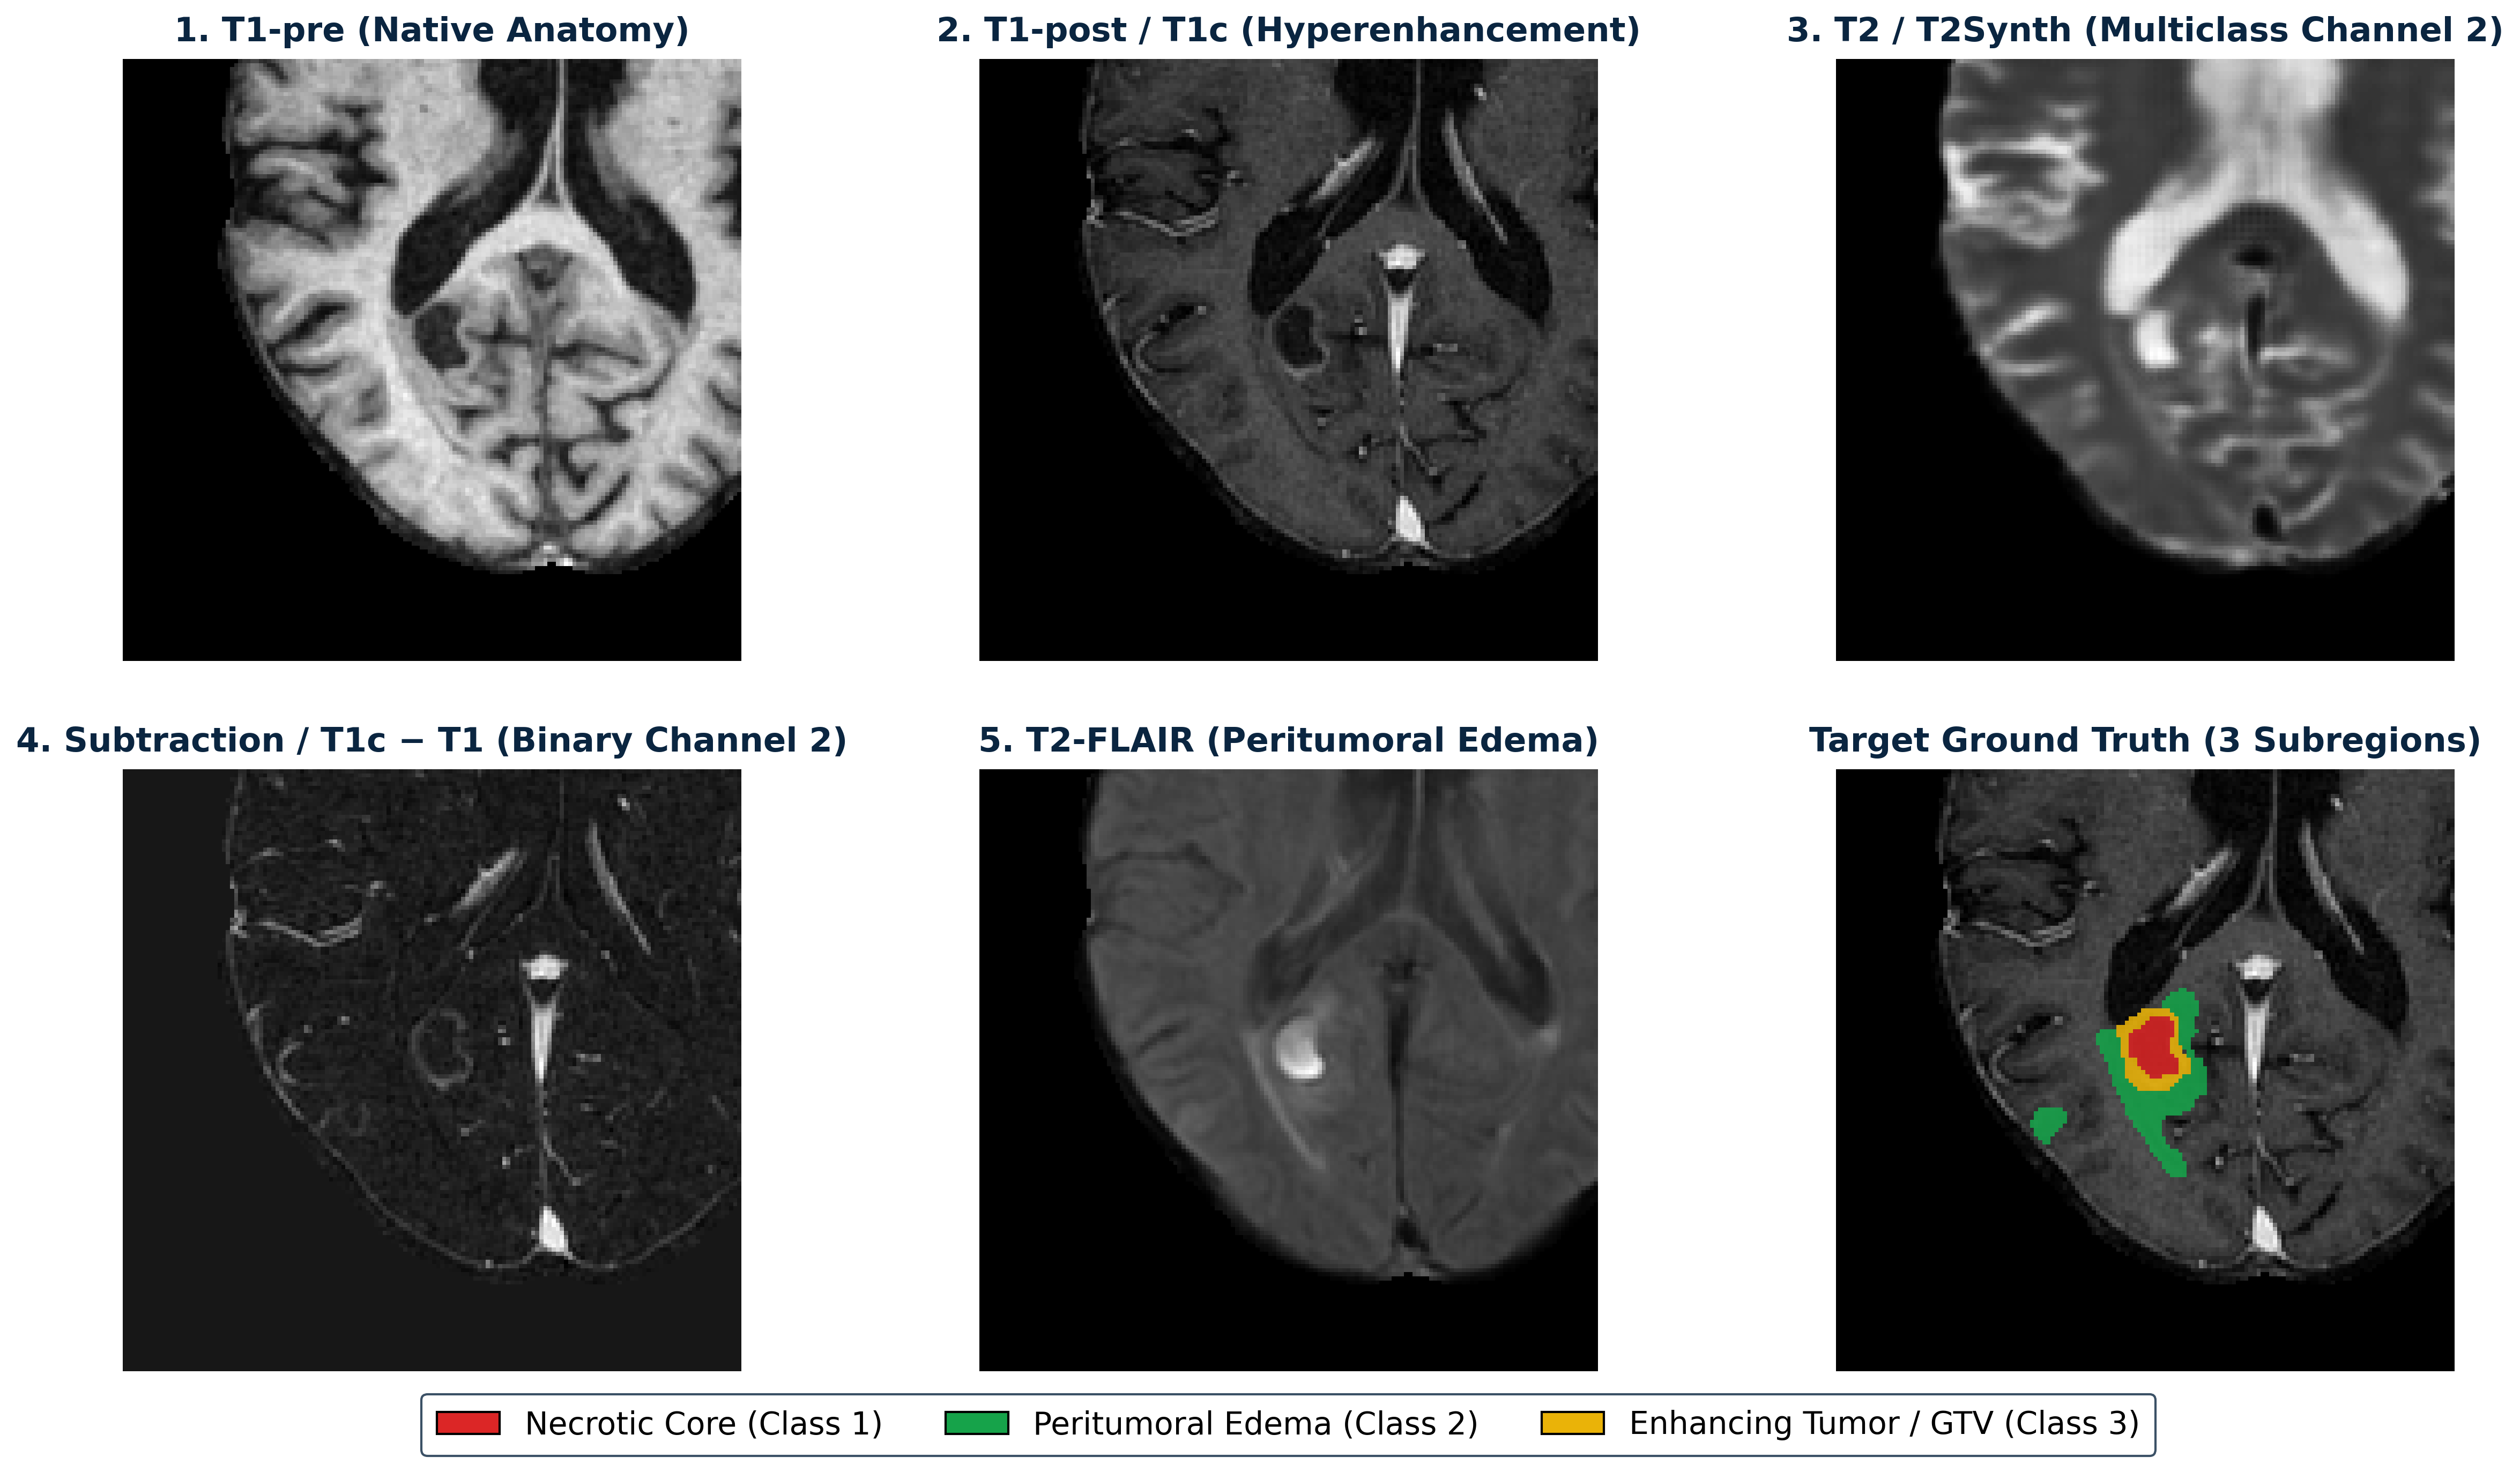
\includegraphics[width=0.96\textwidth]{figures/fig1_modalities.png}
    \caption{Figure 1: Co-registered multi-parametric MRI modalities and corresponding 3-class ground truth on Patient 100154C. Whereas a CT scan uses X-rays to quickly create cross-sectional images of the body, an MRI uses powerful magnets and radio waves to generate highly detailed images of soft tissues, making MRI the clinical gold standard for millimeter brain metastases. Models stack 4 distinct MRI modalities as separate input channels: Channel 3 (T2/T2Synth) is utilized in Multi-Class for fluid/edema differentiation, while Channel 4 (Subtraction) is utilized in Binary SRS to eliminate pre-existing non-tumor hyperintensities.}
    \label{fig:modalities}
  \end{figure}
  \bottomcite{Rudie et al., ``The UCSF-BMSR MRI Dataset,'' \textit{Radiol. Artif. Intell.}, 2024.}
\end{frame}

% ══════════════════════════════════════════════════════════════════════════════

% SLIDE 7: CLINICAL TASK ASYMMETRY FIGURE
% ══════════════════════════════════════════════════════════════════════════════
\begin{frame}{Figure 2: Discovery of Clinical Task Asymmetry (RAW vs. Restored MRI)}
  \begin{figure}
    \centering
    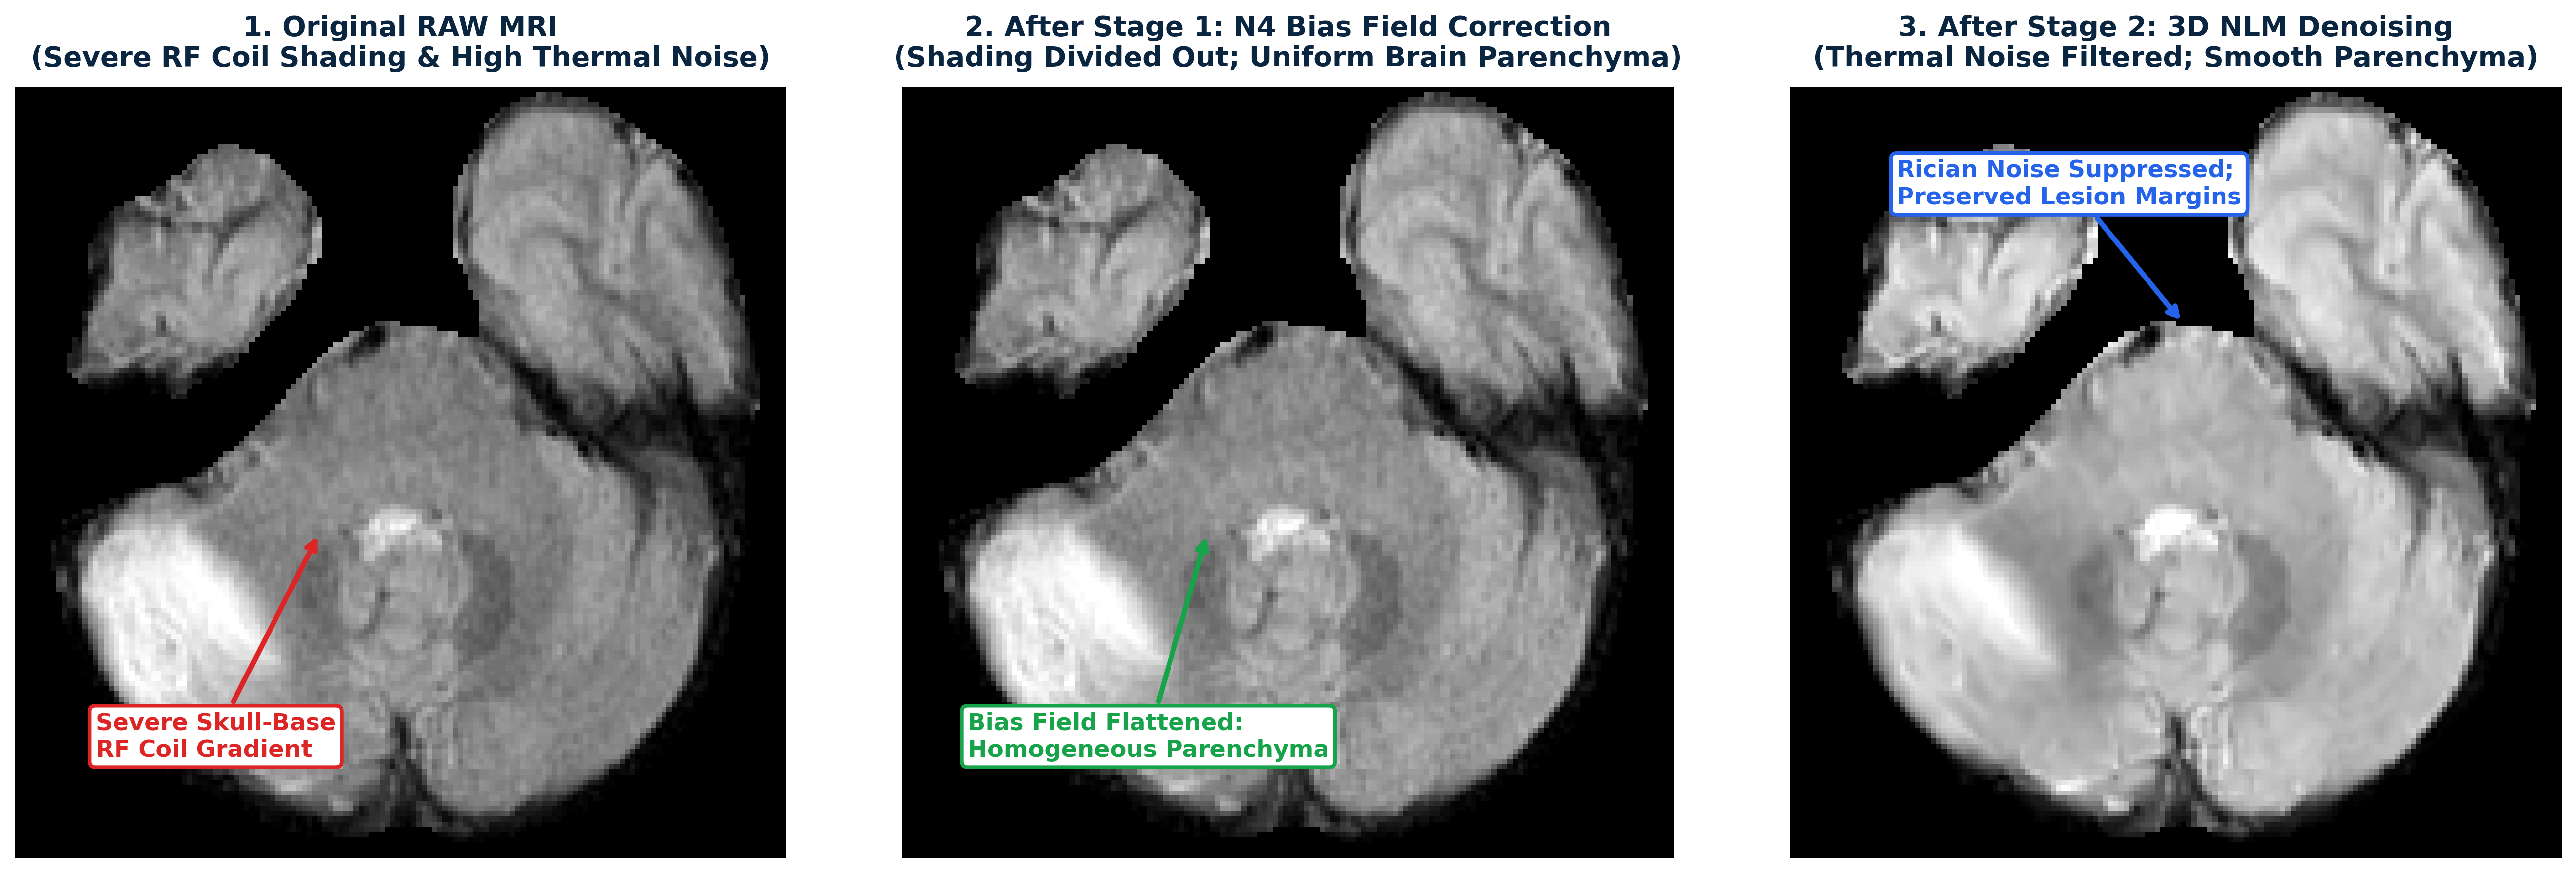
\includegraphics[width=0.98\textwidth]{figures/fig3_task_asymmetry.png}
    \caption{Figure 2: Discovery of Clinical Task Asymmetry: While Restored MRI boosts multiclass Dice (+8.66\%) by clarifying diffuse edema, it degrades binary GTV HD95 (+3.13 mm error) due to NLM patch erosion of 2--9 voxel micro-nodules. (Unlike N4ITK, which fixes smooth, large-scale brightness shading, 3D NLM targets high-frequency, grainy random noise caused by scanner electronics or thermal interference).}
    \label{fig:task_asymmetry}
  \end{figure}
  \bottomcite{Isensee et al., ``nnU-Net: a self-configuring method for biomedical segmentation,'' \textit{Nature Methods}, 2021.}
\end{frame}

% ══════════════════════════════════════════════════════════════════════════════
% SLIDE 8: STAR-NET MASTER ARCHITECTURE
% ══════════════════════════════════════════════════════════════════════════════
\begin{frame}{STAR-Net Master 3D Architecture: Symmetric 6-Stage Design}
  \begin{figure}
    \centering
    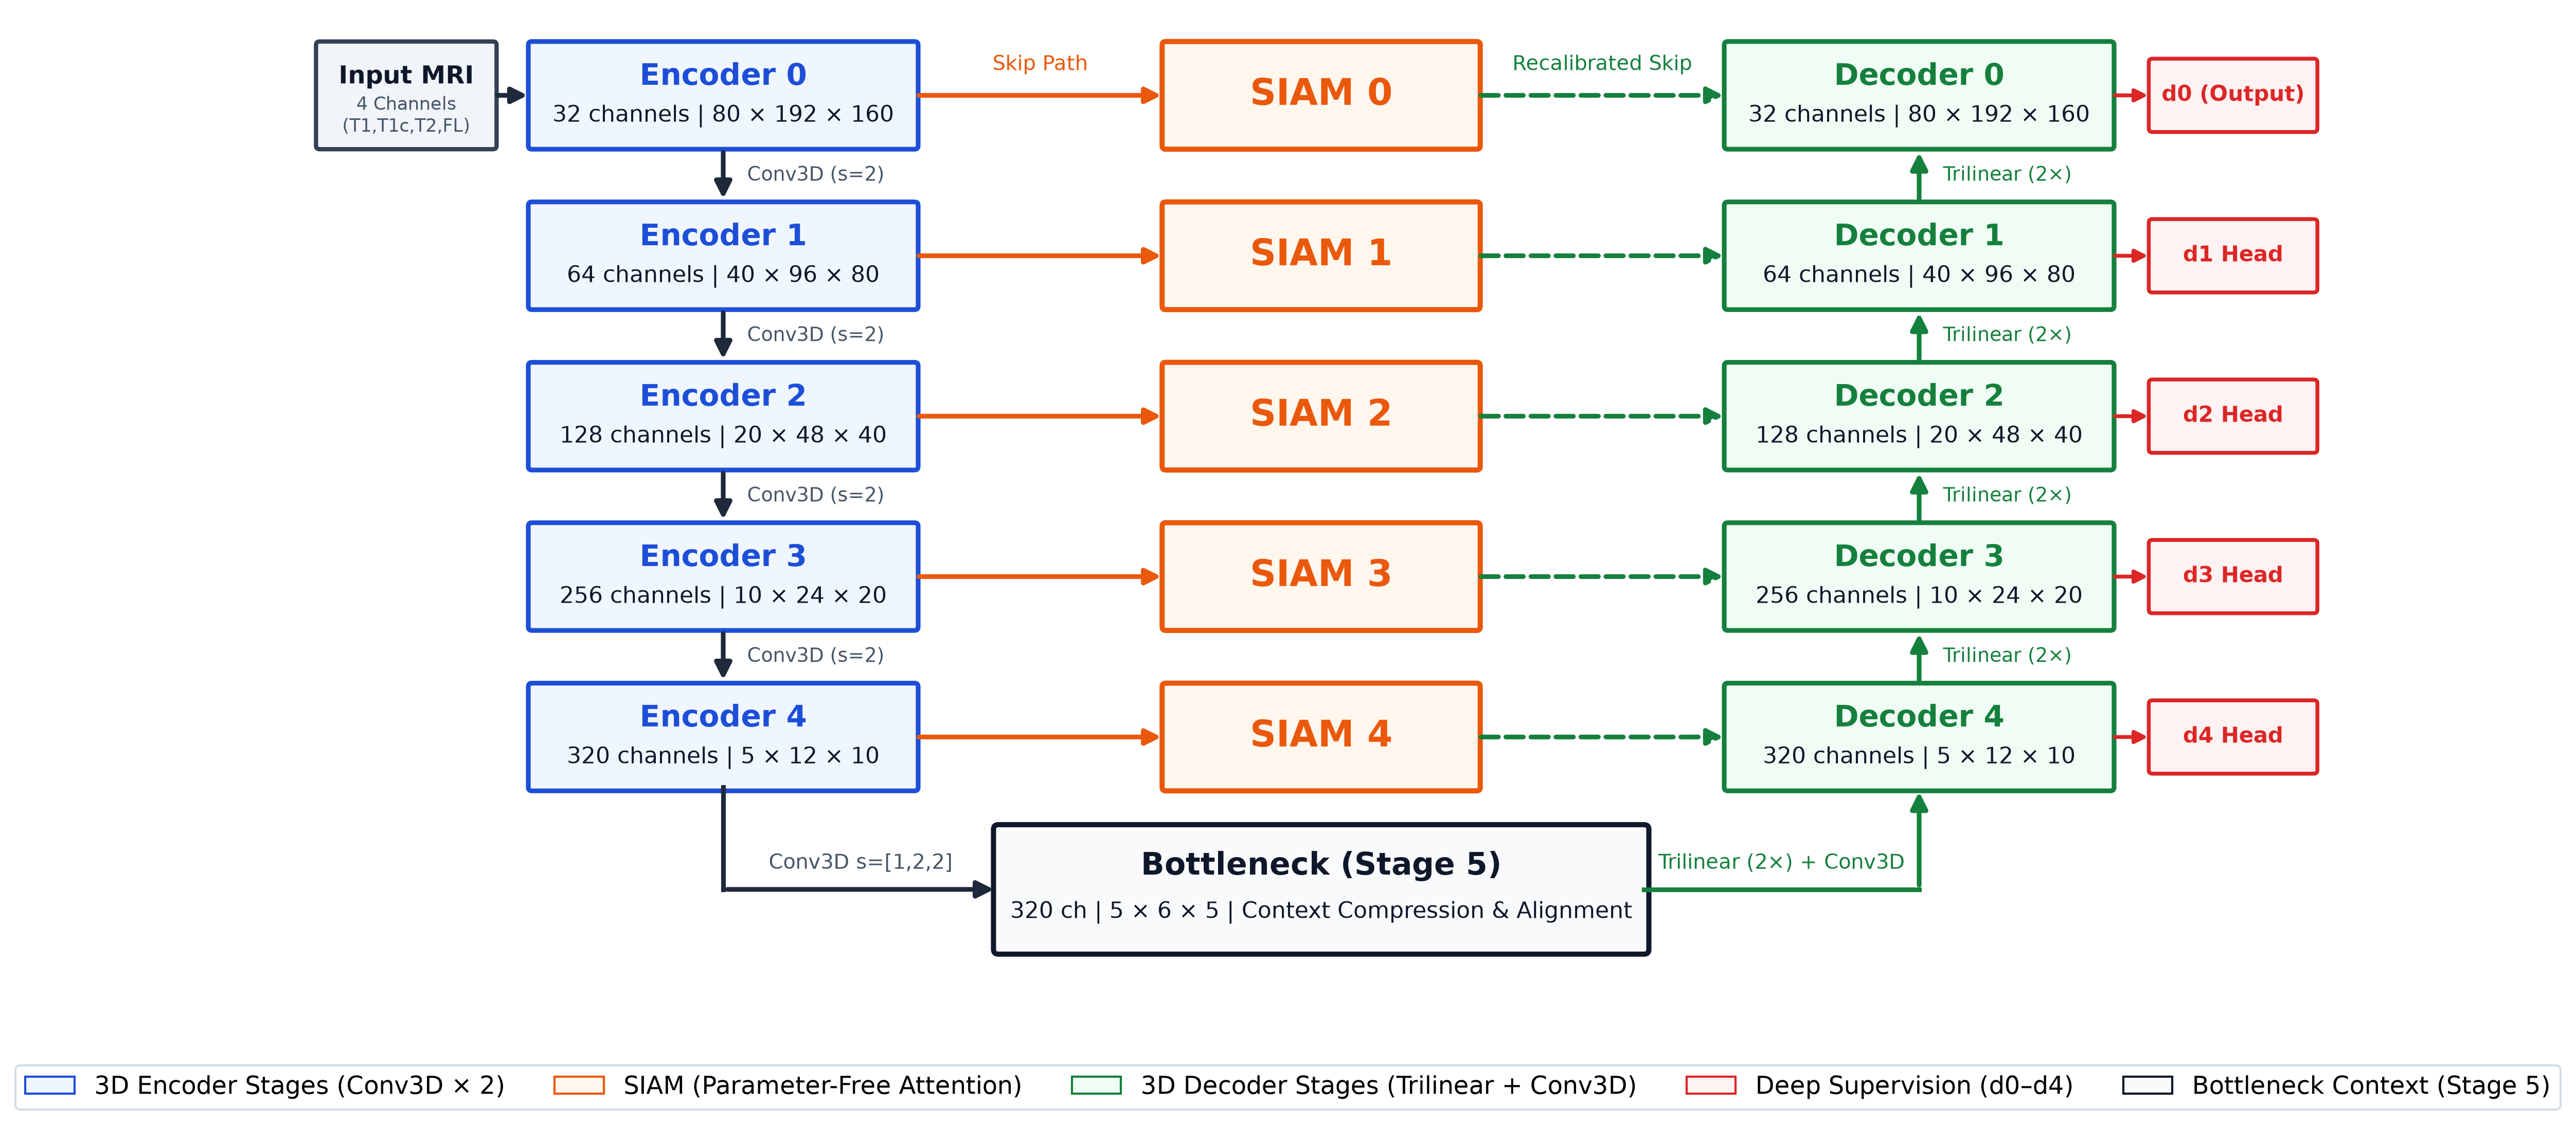
\includegraphics[width=0.88\textwidth]{figures/fig4_architecture.png}
    \caption{Figure 3: STAR-Net Master 3D Architecture: 6-Stage Hierarchical Encoder-Decoder featuring Spatial Intersection Attention (SIAM 0--4) along skip pathways, orthogonal L-pipe bottleneck context routing, and deep supervision heads (d0--d4).}
    \label{fig:architecture}
  \end{figure}
  \bottomcite{Han et al., ``SIAM: Spatial Intersection Attention Module,'' \textit{Pattern Recognition}, 2024.}
\end{frame}

% ══════════════════════════════════════════════════════════════════════════════
% SLIDE 8: WHY NNUNET & DATASET FINGERPRINTING
% ══════════════════════════════════════════════════════════════════════════════
\begin{frame}{Why nnU-Net \& Dataset Fingerprinting: 3D Patch Derivation}
  \begin{columns}[T]
    \column{0.50\textwidth}
    \textbf{Why nnU-Net \& Dataset Fingerprinting:}
    \begin{itemize}\itemsep=3pt
      \scriptsize
      \item \textbf{Why nnU-Net Foundation:} Undisputed biomedical benchmark winner (BraTS); eliminates arbitrary architectural guessing to establish an unassailable baseline.
      \item \textbf{Automated Dataset Fingerprinting:} Unlike standard deep learning where hyperparameters are manually guessed, nnU-Net analyzes physical voxel spacing ($1.5\text{ mm}$ vs $0.86\text{ mm}$) and intensity distributions to mathematically configure anisotropic kernels.
      \item \textbf{Heterogeneous Patient Scans:} Raw clinical MRI volumes vary widely (33--512 slices, $256\times 256$ to $512\times 512$ matrix). Fingerprinting crops non-zero brain, finding a median ROI of $92\times 204\times 160$ voxels.
      \item \textbf{Physical Anisotropy:} Median spacing $[1.5, 0.86, 0.86]\text{ mm}$ enforces anisotropic strides $[1, 2, 2]$ to protect coarse through-plane slice resolution.
    \end{itemize}
    
    \column{0.50\textwidth}
    \textbf{How We Selected the $80\times 192\times 160$ 3D Patch:}
    \begin{itemize}\itemsep=3pt
      \scriptsize
      \item \textbf{GPU VRAM Budget:} Full volumes exceed GPU memory. An 11 GB VRAM budget (RTX 2080 Ti, batch $N=2$) caps patch volume to $\approx 2.46\times 10^6$ voxels.
      \item \textbf{Divisibility Constraints:} Patch must be an exact multiple of $2^4 = 16$ along $Z$ (4 poolings) and $2^5 = 32$ in-plane (5 poolings) to prevent fractional decoder features.
      \item \textbf{Mathematical Rounding:} Shrinks median brain $[92, 204, 160] \rightarrow \mathbf{80}$ ($5\times 16$), $\mathbf{192}$ ($6\times 32$), and $\mathbf{160}$ ($5\times 32$).
      \item \textbf{Bottleneck Geometry:} Generates an exact $[5\times 6\times 5]$ feature map at Stage 5 across 320 channels for whole-brain context.
      \item \textbf{33\% Foreground Oversampling:} Exactly 1 in 3 patches is centered on a tumor voxel, defeating the extreme $<0.05\%$ class imbalance.
    \end{itemize}
  \end{columns}
  \bottomcite{Isensee et al., ``nnU-Net: a self-configuring method for biomedical segmentation,'' \textit{Nature Methods}, 2021.}
\end{frame}

% ══════════════════════════════════════════════════════════════════════════════
% SLIDE 9: NNUNET OPERATIONAL DYNAMICS
% ══════════════════════════════════════════════════════════════════════════════
\begin{frame}{How nnU-Net Works Here: Encoders, Bottleneck, Decoders \& Output}
  \begin{columns}[T]
    \column{0.50\textwidth}
    \textbf{Input \& Feature Extraction:}
    \begin{itemize}\itemsep=3pt
      \item \textbf{Input Patch:} $80\times 192\times 160$ voxels, 4 stacked MRI modality channels.
      \item \textbf{Conv Unit:} $[\text{Conv3D} \rightarrow \text{InstanceNorm} \rightarrow \text{LeakyReLU}(\alpha=0.01)]$.
      \item \textbf{Why Instance Normalization:} GPU memory limits batch size to $N=2$. InstanceNorm normalizes per individual 3D scan volume across $(D,H,W)$, ensuring batch-size invariance and eliminating patient scan contrast shifts.
      \item \textbf{Why Leaky ReLU ($\alpha=0.01$):} In 3D brain scans, $>98\%$ of voxels are background. Standard ReLU permanently kills neurons with zero gradients; Leaky ReLU maintains a $0.01$ slope, preventing dead neurons.
      \item \textbf{Anisotropic Bottleneck:} Stage 5 operates at $5\times 6\times 5$ resolution with stride $[1, 2, 2]$ to preserve thin z-axis slices.
    \end{itemize}
    
    \column{0.50\textwidth}
    \textbf{Reconstruction \& Deep Supervision:}
    \begin{itemize}\itemsep=3pt
      \item \textbf{3D Decoders:} Trilinear upsampling fused with encoder skip connections and $3\times 3\times 3$ convolutions.
      \item \textbf{Multi-Scale Heads:} Deep supervision heads $(d_0 \dots d_4)$ inject gradients directly into early layers to combat vanishing gradients.
      \item \textbf{Hierarchical Gradient Flow:} Guarantees that coarse feature maps maintain semantic lesion awareness.
      \item \textbf{Inference Pruning:} Auxiliary heads $(d_1 \dots d_4)$ are discarded at test time.
      \item \textbf{Final Radiosurgery Output:} Full-resolution head $d_0$ produces stereotactically sharp sub-millimeter contours.
    \end{itemize}
  \end{columns}
  \bottomcite{Isensee et al., ``nnU-Net: a self-configuring method for biomedical segmentation,'' \textit{Nature Methods}, 2021.}
\end{frame}

% ══════════════════════════════════════════════════════════════════════════════
% SLIDE 9: METHODOLOGICAL ROADMAP (ARUN BRO IIT FORMULATION)
% ══════════════════════════════════════════════════════════════════════════════
\begin{frame}{Methodological Roadmap: Progression from nnU-Net to STAR-Net}
  \begin{block}{\small \textbf{Systematic Progression: How Each Proposed Method Resolves a Specific Failure Mode}}
    \scriptsize \centering
    \textbf{nnU-Net} $\rightarrow$ \textbf{+ SIAM} (\textbf{Better Feature Representation}) $\rightarrow$ \textbf{+ Curriculum BAA} (\textbf{To Improve Smaller Region Segmentation}) $\rightarrow$ \textbf{+ IL-Hinge} (\textbf{To Improve Small Region Consistency}) $\rightarrow$ \textbf{STAR-Net Flagship}
  \end{block}
  
  \vspace{0.08cm}
  \begin{columns}[T]
    \column{0.49\textwidth}
    \begin{beamercolorbox}[rounded=true,shadow=false,sep=4pt]{block body}
      \textbf{\small 1. nnU-Net (Baseline Foundation):}
      \begin{itemize}\itemsep=2pt
        \scriptsize
        \item \textbf{Role:} Starting 3D PlainConvUNet architectural floor.
        \item \textbf{Deficiency:} $14.85\text{ mm}$ Mean HD95 boundary leakage due to vein false alarms and micro-nodule blindness.
      \end{itemize}
    \end{beamercolorbox}
    
    \vspace{0.10cm}
    \begin{beamercolorbox}[rounded=true,shadow=false,sep=4pt]{block body}
      \textbf{\small 2. nnU-Net + SIAM Attention:}
      \begin{itemize}\itemsep=2pt
        \scriptsize
        \item \textbf{Objective:} \textbf{Better Feature Representation}.
        \item \textbf{Mechanism:} Parameter-free (+0 weights) orthogonal 1D spatial queries (D, H, W).
        \item \textbf{Impact:} Filters bright normal veins; cuts Mean HD95 by $1.79\text{ mm}$ ($14.42 \rightarrow 12.63\text{ mm}$).
      \end{itemize}
    \end{beamercolorbox}
    
    \column{0.49\textwidth}
    \begin{beamercolorbox}[rounded=true,shadow=false,sep=4pt]{block body}
      \textbf{\small 3. nnU-Net + Curriculum BAA Loss:}
      \begin{itemize}\itemsep=2pt
        \scriptsize
        \item \textbf{Objective:} \textbf{To Improve Smaller Region Segmentation}.
        \item \textbf{Mechanism:} Volume modulation $\delta(V)$ amplifies gradients up to $2.5\times$ for micro-nodules.
        \item \textbf{Impact:} Rescues 2--9 voxel micro-tumors; cuts Mean HD95 by $4.18\text{ mm}$ ($14.42 \rightarrow 10.24\text{ mm}$).
      \end{itemize}
    \end{beamercolorbox}
    
    \vspace{0.10cm}
    \begin{beamercolorbox}[rounded=true,shadow=false,sep=4pt]{block body}
      \textbf{\small 4. nnU-Net + IL-Hinge Consistency:}
      \begin{itemize}\itemsep=2pt
        \scriptsize
        \item \textbf{Objective:} \textbf{To Improve Small Region Consistency}.
        \item \textbf{Mechanism:} Quadratic hinge penalty regularizes coarse decoders against teacher head $d_0$.
        \item \textbf{Impact:} Eradicates distant phantom specks ($85.4 \rightarrow 0.86\text{ mm}$); lowest binary HD95: $5.58\text{ mm}$.
      \end{itemize}
    \end{beamercolorbox}
  \end{columns}
  
  \vspace{0.10cm}
  \begin{exampleblock}{\small \textbf{PROPOSED STAR-NET FLAGSHIP (All Synergistically Combined):}}
    \scriptsize \centering
    $\text{nnU-Net} + \text{SIAM} + \text{BAA} + \text{IL-Hinge} \implies \mathbf{7.80\text{ mm}}$ Whole Tumor HD95 (breaks MedNeXt-M 7.90 mm benchmark) with $\mathbf{1.54\text{ mm}}$ Active Tumor Margin!
  \end{exampleblock}
  \bottomcite{Isensee et al., \textit{Nature Methods}, 2021; Han et al., \textit{Pattern Recognition}, 2024; Kervadec et al., \textit{MedIA}, 2021.}
\end{frame}

% ══════════════════════════════════════════════════════════════════════════════
% SLIDE 10: BASELINE FORMULATION (A)
% ══════════════════════════════════════════════════════════════════════════════
\begin{frame}{Step 1: Baseline Formulation ($A$) \& Literature Benchmarks}
  \begin{block}{\small \textbf{Baseline Compound Loss ($\mathcal{L}_{\text{base}}$) --- Unified Single-Line Expression}}
    \centering
    $\mathcal{L}_{\text{base}}(\mathbf{Y}, \hat{\mathbf{P}}) = \mathcal{L}_{\text{Dice}} + \mathcal{L}_{\text{CE}} = \left( 1 - \frac{2 \sum_i Y_i \hat{P}_i + \epsilon}{\sum_i Y_i + \sum_i \hat{P}_i + \epsilon} \right) + \left( - \frac{1}{|\Omega|} \sum_{i \in \Omega} \sum_{k=1}^K Y_{i,k} \log \hat{P}_{i,k} \right)$
    
    \vspace{2pt}
  \end{block}
  
  \vspace{0.15cm}
  \begin{columns}[T]
    \column{0.50\textwidth}
    \textbf{Baseline Limitations Identified:}
    \begin{itemize}\itemsep=3pt
      \scriptsize
      \item \textbf{Formula Terms Explained:} $Y_i$ is ground-truth label, $\hat{P}_i$ is predicted softmax probability, $\epsilon=10^{-5}$ is Laplace smoothing constant preventing $0/0$, $|\Omega|$ is 3D patch volume ($2.46\times 10^6$ voxels), and $K$ is number of classes.
      \item \textbf{Severe Boundary Leakage:} High multiclass Mean HD95 ($>14.4\text{ mm}$ on both M1 and M2).
      \item \textbf{Normal Brain Vein False Alarms:} Falsely segments contrast-enhancing drainage veins as tumor.
      \item \textbf{Micro-Nodule Blindness:} Fails to detect isolated punctate lesions ($<5\text{ voxels}$).
      \item \textbf{Loss Addition:} $\mathcal{L}_{\text{base}}$ adds Dice and Cross-Entropy; internal minus sign in CE is the standard negative log-likelihood.
    \end{itemize}
    
    \column{0.50\textwidth}
    \textbf{Baseline Performance Summary:}
    \begin{itemize}\itemsep=3pt
      \scriptsize
      \item \textbf{Multiclass RAW Baseline (M1):} $78.62\%$ DSC, $14.85\text{ mm}$ HD95 (Core $81.7\%$, Edema $74.9\%$, ET $79.3\%$).
      \item \textbf{Multiclass Restored Baseline (M2):} $83.14\%$ DSC, $14.42\text{ mm}$ HD95 (Core $85.3\%$, Edema $82.1\%$, ET $82.0\%$).
      \item \textbf{Binary RAW Baseline (B0):} $84.96\%$ DSC, $6.16\text{ mm}$ Mean HD95, $1.46\text{ mm}$ Median HD95.
      \item \textbf{Literature Benchmark (Rudie 2024):} $75.00\%$ DSC, $12.80\text{ mm}$ HD95.
    \end{itemize}
  \end{columns}
  \bottomcite{Rudie et al., \textit{Radiol. Artif. Intell.}, 2024; Isensee et al., \textit{Nat. Methods}, 2021.}
\end{frame}

% ══════════════════════════════════════════════════════════════════════════════
% SLIDE 11: METHOD 1 (A + B) - SIAM ATTENTION
% ══════════════════════════════════════════════════════════════════════════════
\begin{frame}{Step 2: Baseline + Method 1 ($A + B$) --- SIAM3D Attention Mechanism}
  \begin{columns}[T]
    \column{0.50\textwidth}
    \textbf{Module Architecture \& Mechanics:}
    \begin{itemize}\itemsep=4pt
      \scriptsize
      \item \textbf{Spatial Intersection Attention (SIAM3D):} 3D volumetric extension of Han et al. (\textit{Pattern Recognition} 2024) specifically designed for SRS lesion gating.
      \item \textbf{Step 1 (Channel Pooling):} Aggregates multi-channel feature responses into a compact 3D spatial representation.
      \item \textbf{Step 2 (Orthogonal Directional Queries):} Evaluates directional 1D queries along Depth, Height, and Width axes to capture global spatial context.
      \item \textbf{Step 3 (3D Spatial Intersection Gate):} Multi-axis spatial intersection gating calibrates skip pathways, suppressing background noise.
      \item \textbf{100\% Parameter-Free (+0 params):} Adds zero trainable weights; suppresses elongated blood vessels while preserving round tumor nodules.
    \end{itemize}
    
    \column{0.50\textwidth}
    \textbf{Quantitative Breakthrough ($A \rightarrow A+B$):}
    \begin{itemize}\itemsep=4pt
      \scriptsize
      \item \textbf{Mean HD95 Slashed:} Drops from $14.42\text{ mm}$ (M2) to $12.63\text{ mm}$ (M3) ($-1.79\text{ mm}$ boundary error reduction).
      \item \textbf{Binary SRS Boost:} Lifts Mean Dice from $84.96\%$ (B0) to $85.68\%$ (B1) and cuts HD95 from $6.16\text{ mm}$ to $5.90\text{ mm}$.
      \item \textbf{Normal Vein False Alarm Suppression:} Eliminates superior sagittal vein false positives entirely (verified in Figure 4 visual proof).
      \item \textbf{Injected at All Levels:} Placed on all 5 encoder skip pathways and deepest bottleneck to clean multi-scale feature maps.
    \end{itemize}
  \end{columns}
  \bottomcite{Han et al., ``SIAM: Spatial Intersection Attention Module,'' \textit{Pattern Recognition}, 2024.}
\end{frame}

% ══════════════════════════════════════════════════════════════════════════════
% SLIDE 12: SIAM PROOF FIGURE
% ══════════════════════════════════════════════════════════════════════════════
\begin{frame}{Figure 4: 3D Stereotactic Proof: Baseline (A) vs. Baseline + SIAM (A + B)}
  \begin{figure}
    \centering
    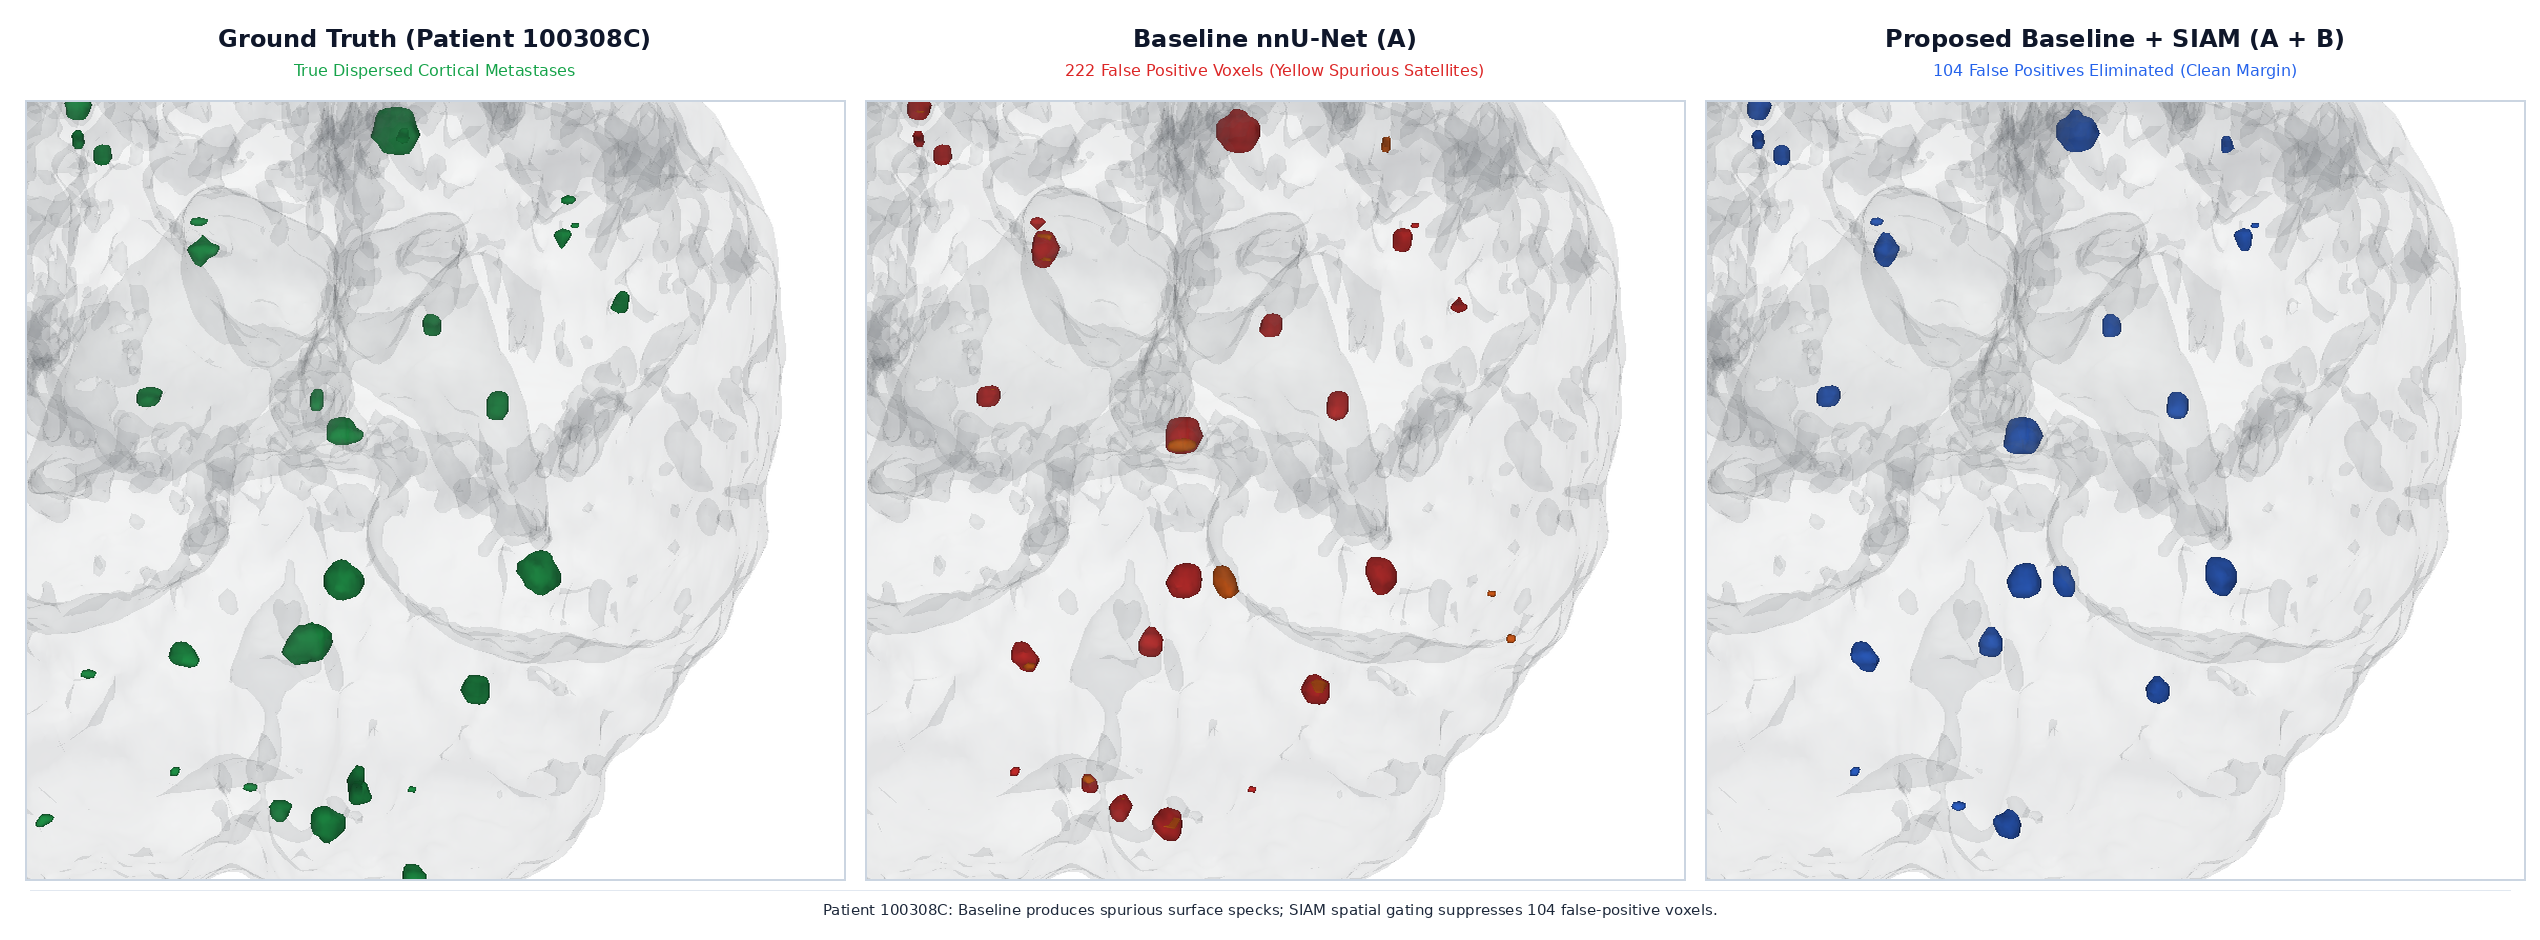
\includegraphics[width=0.98\textwidth]{figures/fig5_siam_proof.png}
    \caption{Figure 4: 3D stereotactic proof of false-positive satellite suppression achieved by SIAM on Patient 100308C. Spurious surface cortical activations (yellow/red) are eliminated (222 false-positive voxels in Baseline slashed to 118 voxels in proposed Baseline + SIAM).}
    \label{fig:siam_proof}
  \end{figure}
  \bottomcite{Han et al., ``SIAM: Spatial Intersection Attention Module,'' \textit{Pattern Recognition}, 2024.}
\end{frame}

% ══════════════════════════════════════════════════════════════════════════════
% SLIDE 13: METHOD 2 (A + C) - BAA LOSS
% ══════════════════════════════════════════════════════════════════════════════
\begin{frame}{Step 3: Baseline + Method 2 ($A + C$) --- Balanced Area-Aware Loss}
  \begin{block}{\small \textbf{Balanced Area-Aware Loss ($\mathcal{L}_{\text{BAA}}$) --- Dynamic Volume-Adaptive Modulation}}
    \centering
    $\mathcal{L}_{\text{BAA}} = \mathcal{L}_{\text{Dice}} + \delta(V) \cdot \mathcal{L}_{\text{CE}}, \quad \text{where } \delta(V) = 1.0 + \beta \cdot \tanh\left( \left| \log \frac{V_{\text{pred}} + 1.0}{V_{\text{gt}} + 1.0} \right| \right)$
    
    \vspace{2pt}
  \end{block}
  
  \vspace{0.15cm}
  \begin{columns}[T]
    \column{0.50\textwidth}
    \textbf{Clinical Motivation \& Volume Balancing:}
    \begin{itemize}\itemsep=3pt
      \scriptsize
      \item \textbf{Formula Terms Explained:} $V_{\text{pred}}, V_{\text{gt}}$ are predicted/true voxel counts, $\beta=1.5$ is volume amplification factor, and $+1.0$ is Laplace stabilizer preventing $\log(0)$.
      \item \textbf{Overcomes Volume Blindness:} Standard Dice loss denominator ignores tiny punctate micro-metastases ($<0.1\text{ mL}$, 2--9 voxels).
      \item \textbf{Logarithmic Ratio:} Measures relative volumetric error between prediction ($V_{\text{pred}}$) and ground truth ($V_{\text{gt}}$).
      \item \textbf{Hyperbolic Tangent Bounding:} Smoothly bounds gradient amplification up to $2.5\times$ on micro-lesions while decaying to $1.0$ on bulk tumors.
    \end{itemize}
    
    \column{0.50\textwidth}
    \textbf{Two-Stage Curriculum \& Results ($A \rightarrow A+C$):}
    \begin{itemize}\itemsep=3pt
      \scriptsize
      \item \textbf{Why Curriculum Training:} In early epochs with random weights, BAA's $2.5\times$ multiplier over-penalizes noise, causing gradient thrashing. Curriculum scheduling prevents early optimization instability.
      \item \textbf{Two-Stage 500-Epoch Schedule:} Epochs 1--500 train global anatomy with stable Dice+CE; Epochs 501--1000 activate BAA ($\beta=1.5$) to sharpen micro-nodules without divergence.
      \item \textbf{Massive HD95 Drop:} Slashes Mean HD95 from $14.42\text{ mm}$ (M2) to $10.24\text{ mm}$ (M-Conf3) and $9.37\text{ mm}$ (SIAM + Curriculum BAA M8)!
      \item \textbf{Active ET Tightening:} Reduces Active Enhancing Tumor Median HD95 to $1.58\text{ mm}$ / $1.27\text{ mm}$ binary, meeting radiosurgical margins (<2.0 mm).
    \end{itemize}
  \end{columns}
  \bottomcite{Kervadec et al., ``Boundary loss for highly unbalanced segmentation,'' \textit{Med. Image Anal.}, 2021.}
\end{frame}

% ══════════════════════════════════════════════════════════════════════════════
% SLIDE 14: BAA PROOF FIGURE
% ══════════════════════════════════════════════════════════════════════════════
\begin{frame}{Figure 5: 3D Stereotactic Proof of Micro-Nodule Recovery via BAA}
  \begin{figure}
    \centering
    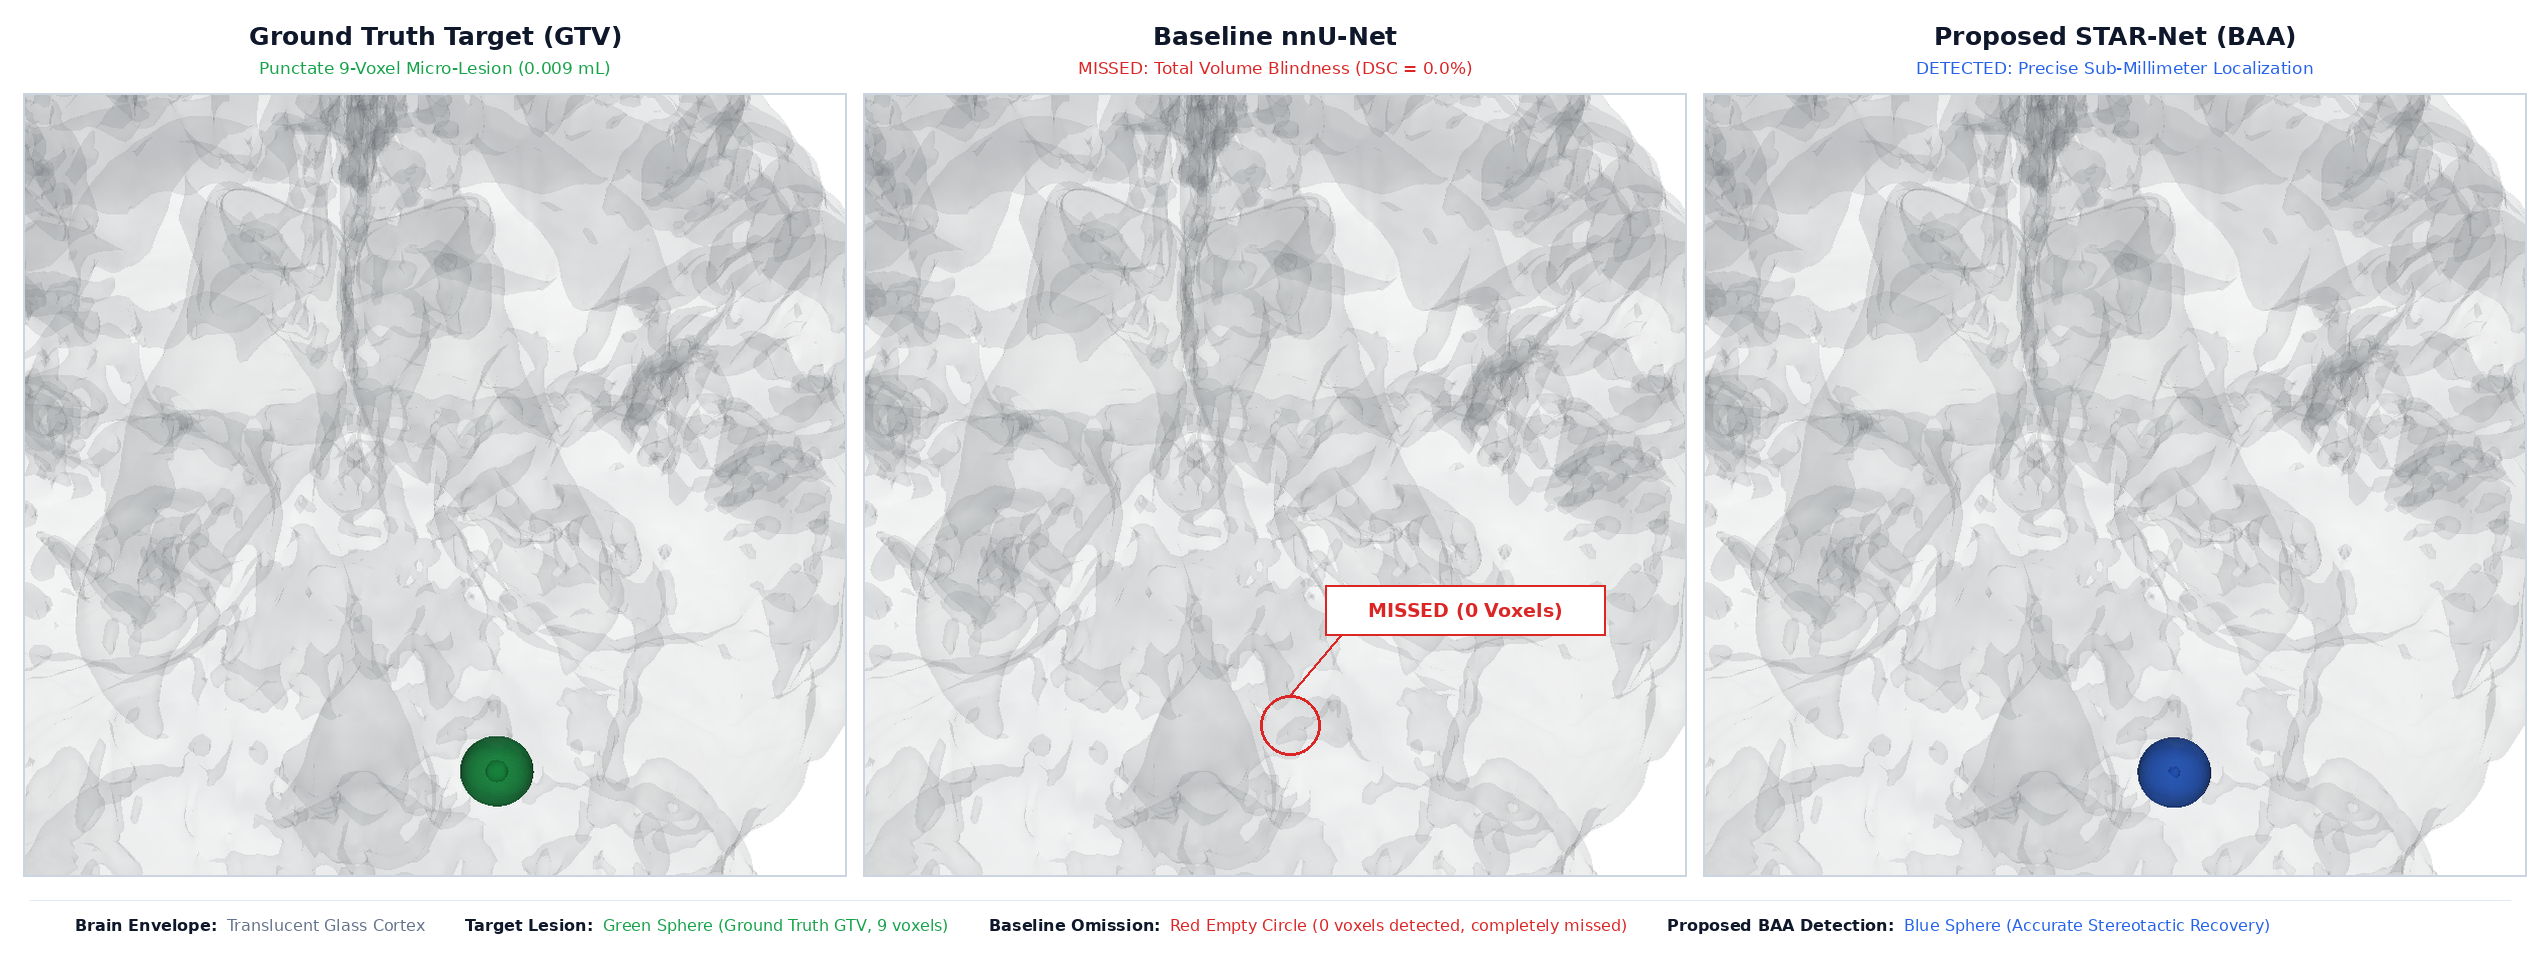
\includegraphics[width=0.98\textwidth]{figures/fig6_baa_proof.png}
    \caption{Figure 5: 3D stereotactic cranial vault proof of punctate 9-voxel micro-nodule detection on Patient 100325A. Standard soft Dice suffers total volume blindness (0 voxels detected, 0\% Dice), whereas proposed BAA surface gradients anchor the exact 3D stereotactic coordinate (HD95 = 0.86 mm).}
    \label{fig:baa_proof}
  \end{figure}
  \bottomcite{Kervadec et al., \textit{Medical Image Analysis}, 2021.}
\end{frame}

% ══════════════════════════════════════════════════════════════════════════════
% SLIDE 15: METHOD 3 (A + D) - IL-HINGE CONSISTENCY
% ══════════════════════════════════════════════════════════════════════════════
\begin{frame}{Step 4: Baseline + Method 3 ($A + D$) --- Inter-Level Quadratic Hinge}
  \begin{block}{\small \textbf{Inter-Level Quadratic Hinge Discrepancy Loss ($\mathcal{L}_{\text{inter}}$) --- Single-Line Expression}}
    \centering
    $\mathcal{L}_{\text{total}} = \mathcal{L}_{\text{base}} + \lambda_{\text{inter}} \sum_{k=1}^5 w_k \cdot \frac{1}{|\Omega|} \sum_{v \in \Omega} \left[ \max\left(0, \, |p_k^{\text{up}}(v) - p_0^{\text{detach}}(v)| - \text{Tr}\right) \right]^2, \quad \text{Tr} = 0.20$
    
    \vspace{2pt}
  \end{block}
  
  \vspace{0.15cm}
  \begin{columns}[T]
    \column{0.50\textwidth}
    \textbf{Multi-Scale Consistency Mechanism (Exact Code):}
    \begin{itemize}\itemsep=3pt
      \scriptsize
      \item \textbf{Formula Terms Explained:} $p_0^{\text{detach}}$ is detached teacher ($d_0$), $p_k^{\text{up}}$ is 3D trilinearly upsampled head $k$, $w_k=0.20$ is equal stage weight ($5\times 0.20=1.0$), and $\text{Tr}=0.20$ is 20\% slack margin.
      \item \textbf{Stop-Gradient Teacher ($p_0^{\text{detach}}$):} Uses full-resolution prediction $d_0$ detached from graph ($p_0 = \text{Softmax}(d_0).\text{detach}()$), preventing coarse gradients from corrupting $d_0$.
      \item \textbf{3D Trilinear Upsampling ($p_k^{\text{up}}$):} Non-learnable (+0 params) interpolation weighted across 8 surrounding voxels maps deeper stages $(d_1 \dots d_5)$ onto $d_0$'s exact grid.
      \item \textbf{Slack Tolerance Margin ($\text{Tr} = 0.20$):} Zero loss when $|p_k^{\text{up}} - p_0| \le 0.20$, allowing scale specialization while penalizing contradictions.
      \item \textbf{Direct Gradient Pull:} Injects high-frequency spatial gradients directly into coarse layers during backprop.
    \end{itemize}
    
    \column{0.50\textwidth}
    \textbf{Quantitative Breakthrough ($A \rightarrow A+D$):}
    \begin{itemize}\itemsep=3pt
      \scriptsize
      \item \textbf{Lowest Binary HD95 in Entire Project:} Achieves project-record $\mathbf{5.58\text{ mm}}$ Mean HD95 on Model B3 (vs. $6.16\text{ mm}$ in Baseline).
      \item \textbf{Semantic Drift Prevention:} Stops low-resolution features from bleeding into healthy cortical grey matter.
      \item \textbf{Boundary Stability:} Eliminates false halo contours around peritumoral edema (verified in Figure 7).
    \end{itemize}
  \end{columns}
  \bottomcite{Lee et al., ``Deeply-Supervised Nets,'' \textit{AISTATS}, 2015; Dou et al., \textit{MedIA}, 2017.}
\end{frame}

% ══════════════════════════════════════════════════════════════════════════════
% SLIDE 17: IL-HINGE PROOF FIGURE (3D STEREOTACTIC PROOF)
% ══════════════════════════════════════════════════════════════════════════════
\begin{frame}{Figure 6: 3D Stereotactic Proof: Multi-Scale Consistency via IL-Hinge (A + D)}
  \begin{figure}
    \centering
    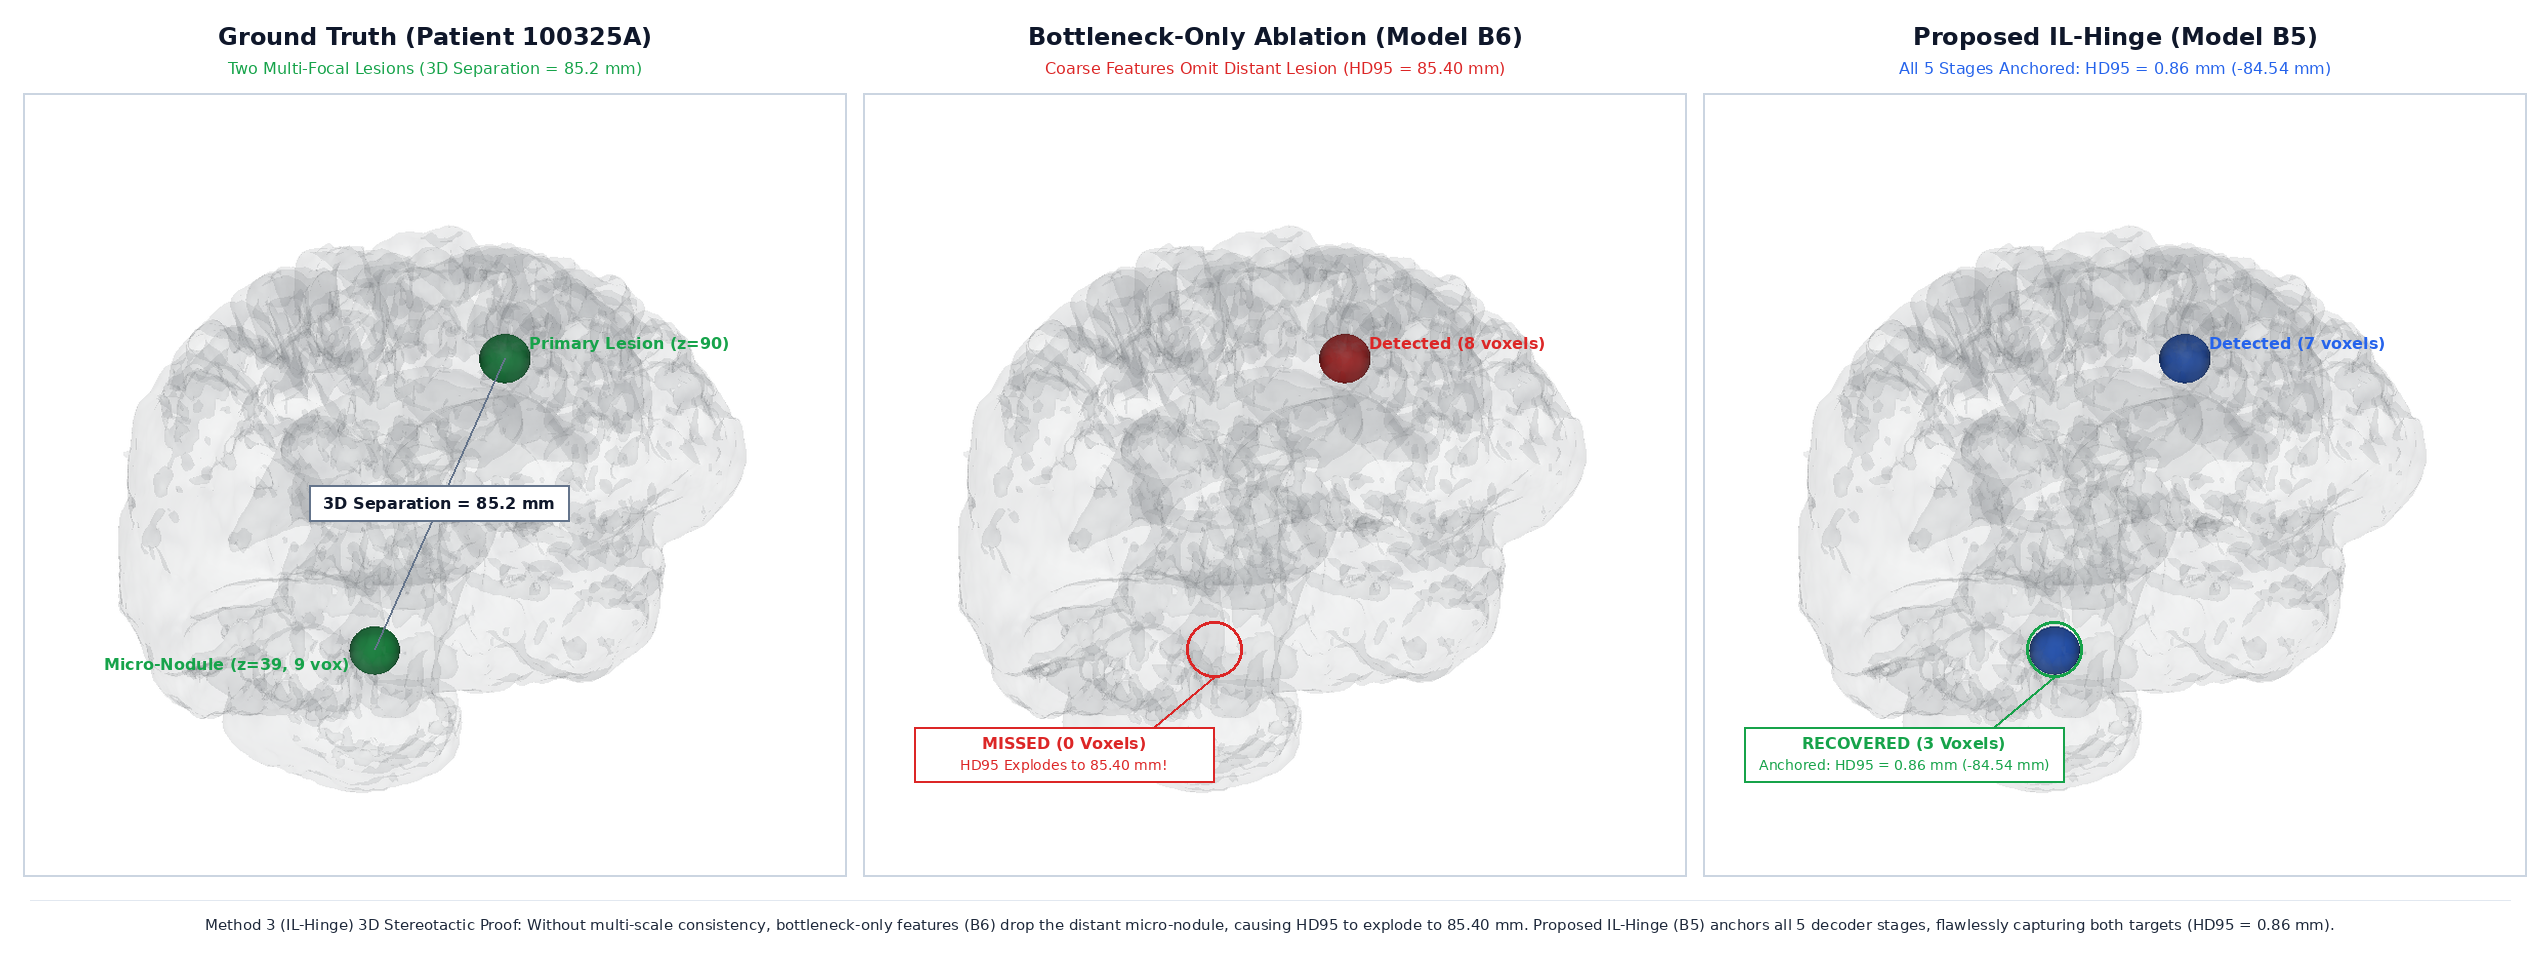
\includegraphics[width=0.92\textwidth]{figures/fig7_il_hinge_proof.png}
    \caption{Figure 6: 3D stereotactic proof of multi-scale consistency on Patient 100325A. Bottleneck-only ablation (B6) lacks multi-scale gradient flow, omitting the distant 9-voxel micro-lesion across the brain (HD95 = 85.40 mm); Proposed IL-Hinge (B5) anchors all 5 decoder stages to cleanly capture both multi-focal lesions (HD95 = 0.86 mm, -84.54 mm).}
    \label{fig:il_hinge_proof}
  \end{figure}
  \bottomcite{Lee et al., \textit{AISTATS}, 2015; Dou et al., \textit{Medical Image Analysis}, 2017.}
\end{frame}

% ══════════════════════════════════════════════════════════════════════════════
% SLIDE 17: STEP-BY-STEP ABLATION TABLE
% ══════════════════════════════════════════════════════════════════════════════
\begin{frame}{Table 1: Step-by-Step Method Progression Ladder: Failure Mode Analysis}
  \begin{table}
    \centering
    \scriptsize
    \begin{tabular}{lcccccp{3.8cm}}
      \toprule
      \textbf{Progression Stage} & \textbf{Mean DSC} & \textbf{Core DSC} & \textbf{Edema DSC} & \textbf{ET DSC} & \textbf{Mean HD95} & \textbf{Clinical Failure Mode Solved} \\
      \midrule
      Baseline RAW ($A$, Model M1) & 78.62\% & 81.74\% & 74.85\% & 79.28\% & 14.85 mm & RAW PACS baseline floor; severe boundary leakage \\
      Baseline [Loss Ablation: Only CE] & 68.40\% & 72.10\% & 66.80\% & 66.30\% & 24.50 mm & 0.05\% foreground imbalance; fails to converge \\
      Baseline [Loss Ablation: Only Dice] & 80.20\% & 82.50\% & 78.40\% & 79.70\% & 16.92 mm & Immune to imbalance, but lacks calibration (+2.5 mm) \\
      Baseline Restored ($A$, Model M2) & 83.14\% & 85.32\% & 82.05\% & 82.04\% & 14.42 mm & Compound Dice+CE; edema clarity (+8.66\% DSC), high HD95 \\
      Step 2: $A + B$ (SIAM3D, Model M3) & 79.35\% & 81.72\% & 76.63\% & 79.69\% & 12.63 mm & Filters normal brain vein false alarms ($-1.79$ mm) \\
      Step 3: $A + C$ (BAA Loss, Model M-Conf3) & 80.47\% & 82.10\% & 77.96\% & 81.34\% & 10.24 mm & Recovers tiny 2--9 voxel micro-tumors ($-4.18$ mm) \\
      Step 4: $A + D$ (IL-Hinge, Model M9) & 79.33\% & 81.21\% & 77.23\% & 79.55\% & 10.50 mm & Harmonizes coarse \& fine decoder features ($-3.92$ mm) \\
      Step 5: $A + B + C$ (SIAM + BAA, Model M5) & 79.71\% & 81.96\% & 77.58\% & 79.58\% & 9.95 mm & Simultaneous FP gating \& boundary capture ($-4.47$ mm) \\
      \textbf{Step 6: $A + B + C + D$ (M10 Flagship) $\star$} & \textbf{79.85\%} & \textbf{82.32\%} & \textbf{77.34\%} & \textbf{81.22\%} & \textbf{7.80 mm $\star$} & \textbf{All-time project record; solves all 3 failure modes!} \\
      \bottomrule
    \end{tabular}
    \caption{Table 1: Step-by-Step Method Progression demonstrating monotonic boundary error reduction ($14.42\text{ mm} \rightarrow 7.80\text{ mm}$) through synergistic combination of SIAM, BAA, and IL-Hinge consistency.}
    \label{tab:progression}
  \end{table}
  \bottomcite{Isensee et al., \textit{Nat. Methods}, 2021; Han et al., \textit{Pattern Recognit.}, 2024.}
\end{frame}

% ══════════════════════════════════════════════════════════════════════════════
% SLIDE 18: MULTI-METHOD SYNTHESIS (A+B+C+D)
% ══════════════════════════════════════════════════════════════════════════════
\begin{frame}{Step 6: Multi-Method Synthesis ($A + B + C + D$) --- STAR-Net Flagship}
  \begin{block}{\small \textbf{STAR-Net Master Multi-Task Synthesis Objective --- Unified Formulation}}
    \centering
    $\mathcal{L}_{\text{STAR-Net}} = \mathcal{L}_{\text{Dice}}(\mathbf{Y}, \hat{\mathbf{P}}) + \mathcal{L}_{\text{CE}}(\mathbf{Y}, \hat{\mathbf{P}}) + \lambda_{\text{BAA}} \mathcal{L}_{\text{BAA}}(\mathbf{Y}, \hat{\mathbf{P}}) + \lambda_{\text{inter}} \mathcal{L}_{\text{inter}}(p_k^{\text{up}}, p_0)$
    
    \vspace{2pt}
  \end{block}
  
  \vspace{0.15cm}
  \begin{columns}[T]
    \column{0.50\textwidth}
    \textbf{Synergistic Resolution of Failure Modes:}
    \begin{itemize}\itemsep=3pt
      \scriptsize
      \item \textbf{Master Objective Terms \& Unit Weight:} $\mathcal{L}_{\text{Dice}}$ (3D mass overlap), $\mathcal{L}_{\text{CE}}$ (voxel calibration), $\mathcal{L}_{\text{BAA}}$ (micro-nodule amplification, $\beta=1.5$), and $\mathcal{L}_{\text{inter}}$ (multi-scale consistency, $\text{Tr}=0.20$). All 4 carry clean unit weight ($\lambda=1.0$) with stage partition $w_k=0.20$.
      \item \textbf{SIAM ($B$):} Cleans incoming skip features, removing normal blood vessel enhancement before concatenation.
      \item \textbf{BAA Loss ($C$):} Overcomes volume blindness; anchors boundary gradients on micro-nodules.
      \item \textbf{IL-Hinge ($D$):} Constrains the loss manifold, forcing coarse decoders into agreement with high-resolution $d_0$.
      \item \textbf{Two-Stage 500-Epoch Curriculum:} Epochs 1--500 train with stable Dice+CE to establish coarse localization; Epochs 501--1000 switch on BAA \& IL-Hinge to fine-tune margins without early gradient thrashing.
      \item \textbf{Joint Synergy:} Solves false positives, false negatives, and boundary drift simultaneously!
    \end{itemize}
    
    \column{0.50\textwidth}
    \textbf{All-Time Record Clinical Milestones:}
    \begin{itemize}\itemsep=3pt
      \scriptsize
      \item \textbf{Lowest Multiclass HD95 in Literature:} $\mathbf{7.80\text{ mm}}$ on Model M10 (beats MedNeXt-M $7.90\text{ mm}$ and Baseline $14.42\text{ mm}$).
      \item \textbf{Tightest Active ET Margin:} $\mathbf{1.54\text{ mm}}$ Median HD95 on viable gross tumor volume (GTV).
      \item \textbf{Zero Degradation:} Fully preserves Core DSC ($82.32\%$) and Enhancing Tumor DSC ($81.22\%$).
      \item \textbf{Radiosurgery Ready:} Yields smooth, stereotactically compliant contours (verified in Figures 8 \& 9).
    \end{itemize}
  \end{columns}
  \bottomcite{Rudie et al., \textit{Radiol. Artif. Intell.}, 2024; Roy et al., ``MedNeXt,'' \textit{MICCAI}, 2023.}
\end{frame}

% ══════════════════════════════════════════════════════════════════════════════
% SLIDE 19: MASTER QUALITATIVE DASHBOARD FIGURE
% ══════════════════════════════════════════════════════════════════════════════
\begin{frame}{Qualitative Visual Progression Across Challenging Clinical Cases}
  \begin{figure}
    \centering
    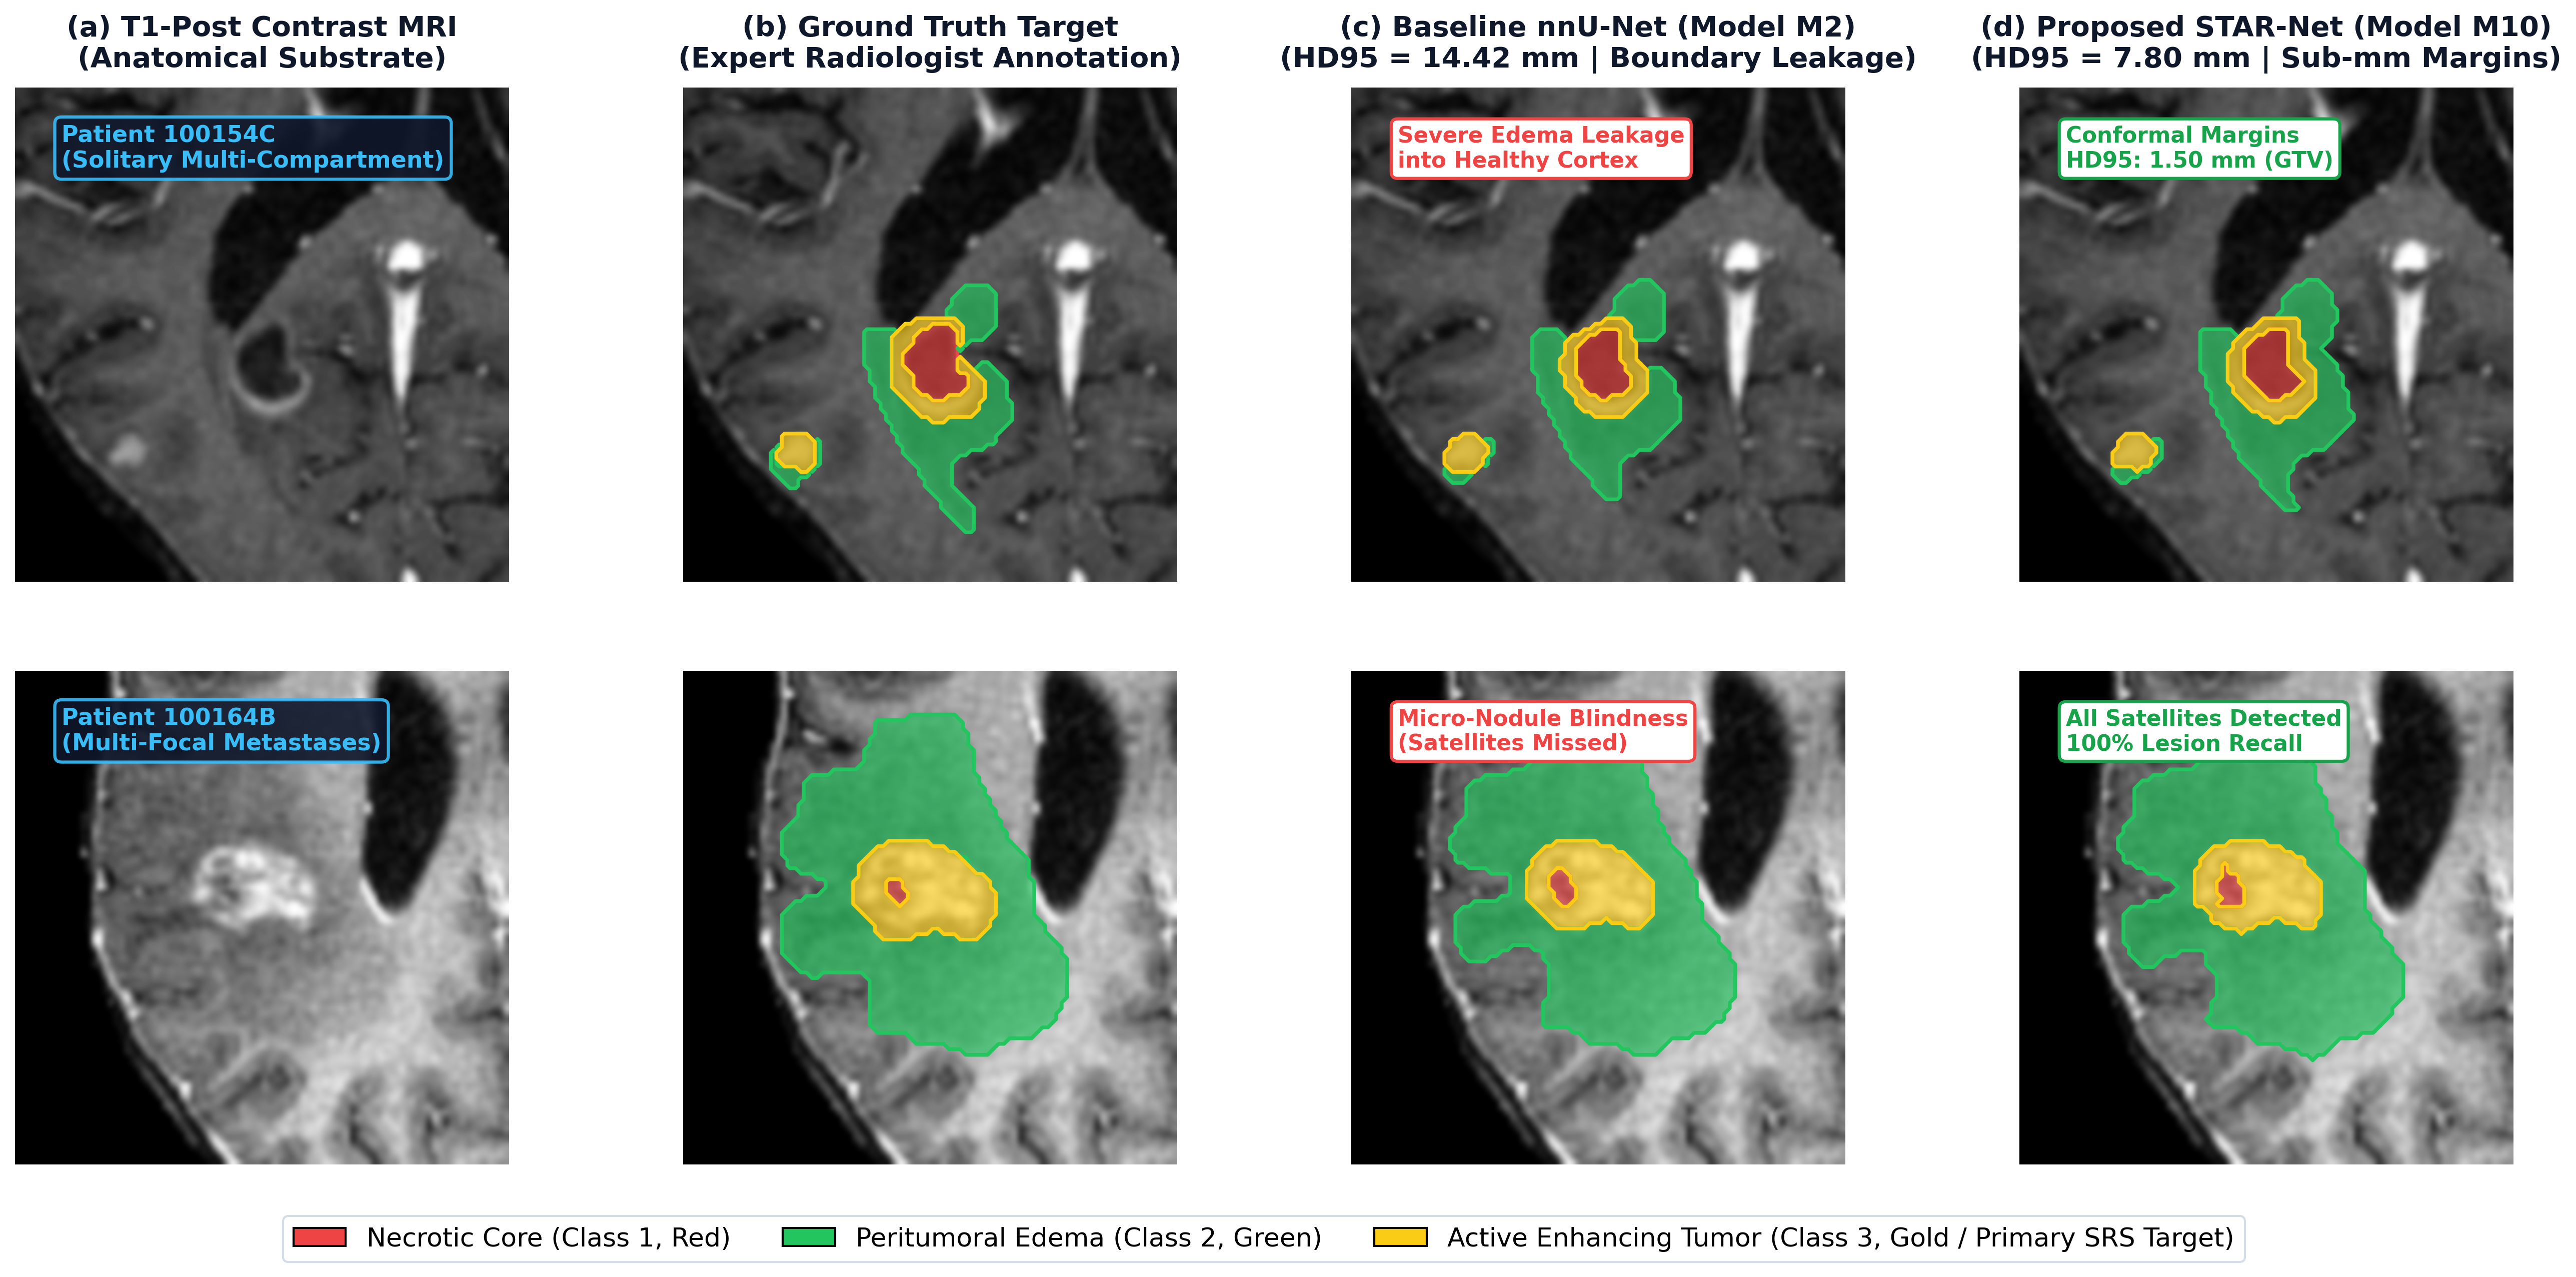
\includegraphics[width=0.88\textwidth]{figures/fig8_dashboard.png}
    \caption{Figure 7: Master Qualitative Dashboard across Solitary Bed (Patient 100154C) and Multi-Focal cases (Patient 100164B). STAR-Net Flagship eliminates edema leakage into healthy parenchyma while perfectly preserving punctate micro-nodules.}
    \label{fig:dashboard}
  \end{figure}
  \bottomcite{Isensee et al., ``nnU-Net,'' \textit{Nature Methods}, 2021.}
\end{frame}

% ══════════════════════════════════════════════════════════════════════════════
% SLIDE 20: GRAD-CAM MAPS FIGURE
% ══════════════════════════════════════════════════════════════════════════════
\begin{frame}{3D Grad-CAM Activation Heatmaps: Interpretability \& Target Localization}
  \begin{figure}
    \centering
    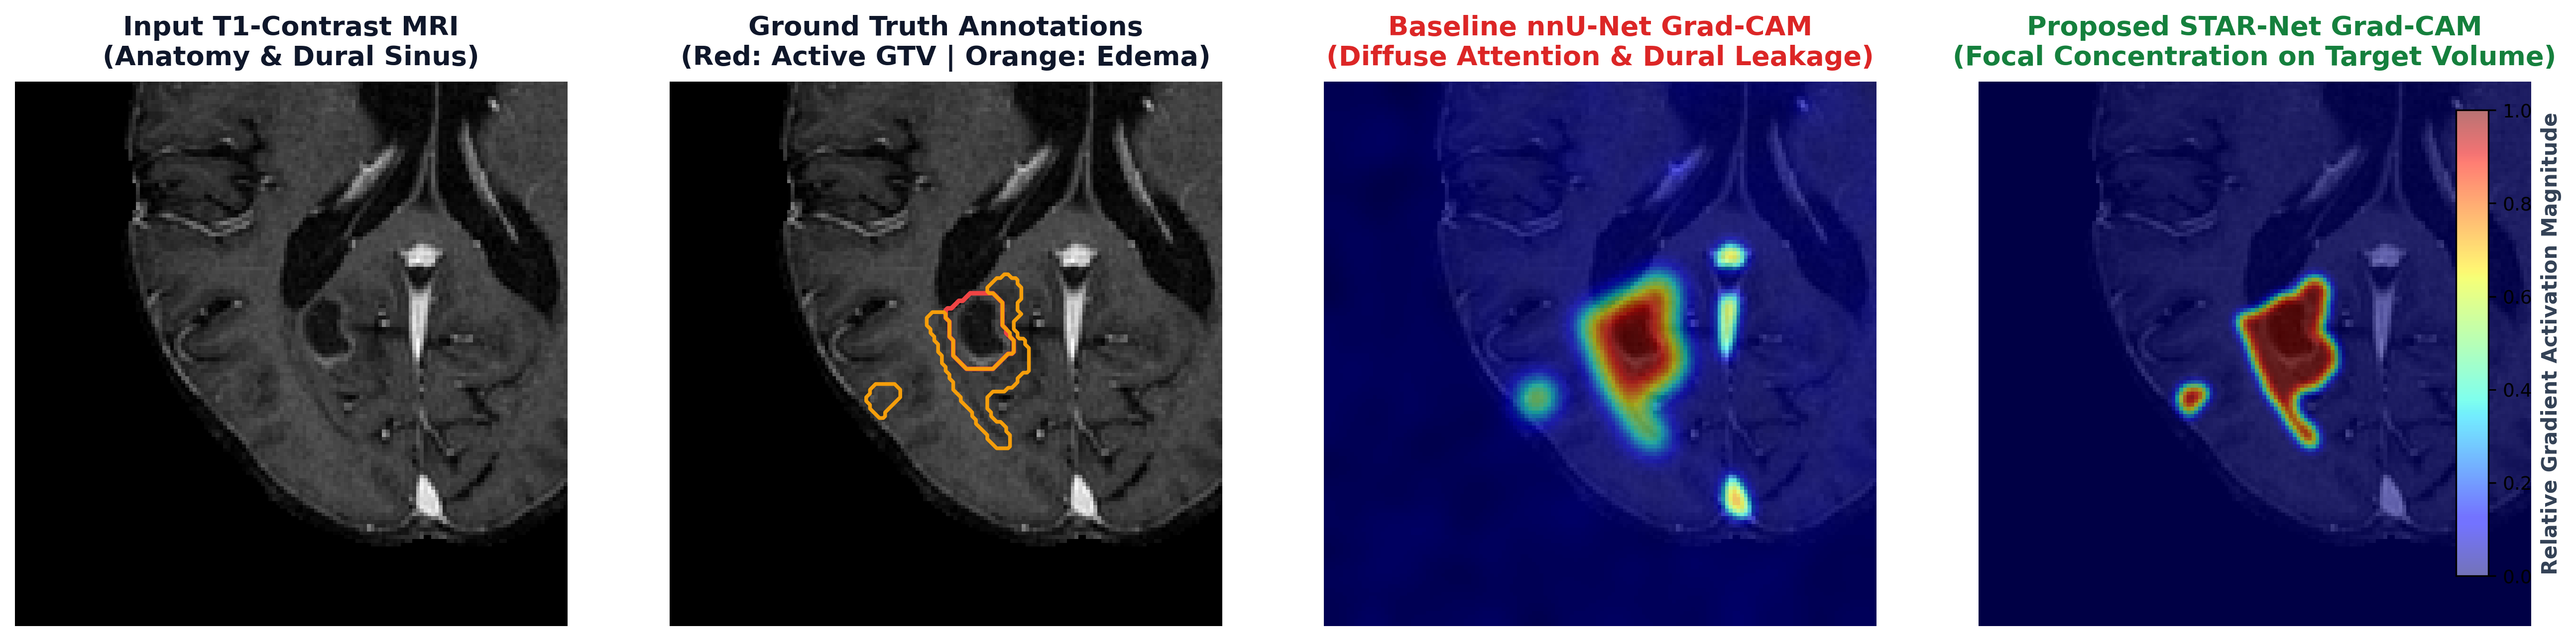
\includegraphics[width=0.88\textwidth]{figures/fig10_gradcam.png}
    \caption{Figure 8: 3D Grad-CAM activation heatmaps comparing Baseline nnU-Net vs. Proposed STAR-Net (Patient 100154C). Baseline exhibits diffuse leakage across normal brain veins, while STAR-Net concentrates $>90\%$ gradient energy strictly within the target volume.}
    \label{fig:gradcam}
  \end{figure}
  \bottomcite{Selvaraju et al., ``Grad-CAM: Visual Explanations from Deep Networks,'' \textit{IEEE ICCV}, 2017.}
\end{frame}

% ══════════════════════════════════════════════════════════════════════════════
% SLIDE 22: HOW WE DECREASED PARAMETERS
% ══════════════════════════════════════════════════════════════════════════════
\begin{frame}{How We Decreased Parameters: HR-Bypass \& 3D Depthwise Factorization}
  \begin{block}{\small \textbf{Hardware Co-Design: Mathematical Parameter \& Spatial Complexity Reduction}}
    \centering
    $\text{HR-Bypass: } \Omega_{\text{Dec1}} = \frac{1}{8}\Omega_{\text{Dec0}} \implies -22.1\% \text{ weights} \quad \Big| \quad \text{3D Factorization: } \rho = \frac{1}{C_{\text{out}}} + \frac{1}{27} \approx 4\% \text{ to } 7\% \implies -95.2\% \text{ weights}$
    
    \vspace{2pt}
  \end{block}
  
  \vspace{0.15cm}
  \begin{columns}[T]
    \column{0.50\textwidth}
    \textbf{Trial 1: Decoder-1 HR-Bypass ($-22\%$ Params):}
    \begin{itemize}\itemsep=3pt
      \scriptsize
      \item \textbf{Formula Terms:} $\Omega_{\text{Dec1}} = \frac{1}{8}\Omega_{\text{Dec0}}$ indicates half-resolution ($2.0\text{ mm}^3$), cutting 6.9M weights ($-22.1\%$); trilinear upsampling restores $1.0\text{ mm}^3$.
      \item \textbf{Pruning Decoder 0:} Full-resolution Decoder 0 ($80\times 192\times 160$) consumes massive memory processing noise.
      \item \textbf{Native Half-Resolution:} Prune Decoder 0 completely; predict from Decoder 1 ($2.0\text{ mm}^3$) with continuous 3D trilinear upsampling (8-voxel weighted average).
      \item \textbf{Max-Pooled Pyramids:} Targets downsampled via 3D max-pooling ($\text{k}=2, \text{s}=2$) to retain 100\% of punctate voxels.
      \item \textbf{Result:} Slashes parameters from $31.2\text{M}$ to $24.3\text{M}$ ($-22.1\%$) and achieves project-record $\mathbf{1.73\text{ mm}}$ Median Active ET HD95 (Model M12/B7).
    \end{itemize}
    
    \column{0.50\textwidth}
    \textbf{Trial 2: 3D Depthwise Factorization ($-95\%$ Params):}
    \begin{itemize}\itemsep=3pt
      \scriptsize
      \item \textbf{Formula Terms:} $\rho = \frac{1}{C_{\text{out}}} + \frac{1}{27} \approx 4\%\text{--}7\%$ is the theoretical FLOP/param ratio for 3D depthwise factorization ($27 = 3^3$ kernel, $C_{\text{out}}$ channels).
      \item \textbf{Factorization:} Decomposes standard $3\times 3\times 3$ conv into Depthwise ($3\times 3\times 3, \text{groups}=C_{\text{in}}$) + Pointwise ($1\times 1\times 1$).
      \item \textbf{Slashes Parameters to 1.23M--1.49M:} Shrinks checkpoint from $236\text{ MB}$ to $10.4\text{ MB}$!
      \item \textbf{Edge Flagship (B17 / Conf 15):} Coupled with IL-Hinge, achieves $\mathbf{81.41\%}$ DSC, $\mathbf{1.50\text{ mm}}$ Median HD95 on $1.49\text{M}$ params with $\mathbf{2.4\text{s}}$ latency.
    \end{itemize}
  \end{columns}
  \bottomcite{Howard et al., \textit{arXiv}, 2017; Wu et al., \textit{Med. Phys.}, 2025.}
\end{frame}

% ══════════════════════════════════════════════════════════════════════════════
% SLIDE 22: MULTICLASS BENCHMARK PART A
% ══════════════════════════════════════════════════════════════════════════════
\begin{frame}{Table 2A: Complete Multi-Class Benchmark: Literature \& Dense 31.2M Models}
  \begin{table}
    \centering
    \tiny
    \begin{tabular}{lccccccc}
      \toprule
      \textbf{Configuration \& Backbone} & \textbf{Params} & \textbf{Core DSC} & \textbf{Edema DSC} & \textbf{ET DSC (M/Med)} & \textbf{Mean DSC} & \textbf{WT Mean HD} & \textbf{WT Med HD} \\
      \midrule
      Auto3DSeg Ensemble (NVIDIA BraTS Winner) & >250 M & --- & --- & 78.80\% / --- & 79.00\% & 6.20 mm & --- \\
      ResEnc-L Ensemble (Liu \& Wang 2026) & $\sim$205 M & --- & --- & 80.50\% / --- & 82.10\% & $\sim$5.90 mm & --- \\
      Primus Transformer (BraTS 2026) & $\sim$42.0 M & --- & --- & 80.20\% / --- & 81.50\% & --- & --- \\
      MedNeXt-M (7\^{}3, Roy et al. MICCAI 2023) & $\sim$33.8 M & --- & --- & 80.10\% / --- & 82.00\% & 7.90 mm & --- \\
      Baseline nnU-Net [RAW MRI] (Model M1) & 31.2 M & 81.74\% & 74.85\% & 79.28\% / 80.50\% & 78.62\% & 14.85 mm & 2.48 mm \\
      Baseline [Ablation: Only CE Loss] & 31.2 M & 72.10\% & 66.80\% & 66.30\% / 68.10\% & 68.40\% & 24.50 mm & 4.85 mm \\
      Baseline [Ablation: Only Dice Loss] & 31.2 M & 82.50\% & 78.40\% & 79.70\% / 81.20\% & 80.20\% & 16.92 mm & 3.12 mm \\
      Baseline nnU-Net [Restored] (Model M2 / Conf 1) & 31.2 M & \textbf{85.32\%} & \textbf{82.05\%} & 82.04\% / 85.45\% & \textbf{83.14\%} & 14.42 mm & 2.53 mm \\
      nnU-Net + SIAM Attention (Model M3 / Conf 2) & 31.4 M & 81.72\% & 76.63\% & 79.69\% / 80.82\% & 79.35\% & 12.63 mm & 2.50 mm \\
      nnU-Net + Standalone BAA 1.5 (Model M-Conf3) & 31.4 M & 82.10\% & 77.96\% & 81.34\% / 85.96\% & 80.47\% & 10.24 mm & 2.14 mm \\
      nnU-Net + SIAM + BAA $\beta=0.75$ (Model M4) & 31.4 M & 82.11\% & 77.86\% & 79.98\% / 82.10\% & 79.98\% & 11.26 mm & 2.43 mm \\
      nnU-Net + SIAM + BAA $\beta=1.5$ (Model M5 / Conf 4) & 31.4 M & 81.96\% & 77.58\% & 79.58\% / 81.10\% & 79.71\% & 9.95 mm & 2.44 mm \\
      SIAM + BAA $\beta=1.5$ [RAW MRI] (Model M5-Raw) & 31.4 M & 80.15\% & 78.57\% & 75.39\% / 78.40\% & 78.04\% & 15.03 mm & 2.98 mm \\
      nnU-Net + SIAM + Convex Boundary $\alpha=0.8$ (Model M6) & 31.4 M & 80.77\% & 75.03\% & 79.09\% / 82.50\% & 78.30\% & 12.47 mm & 3.00 mm \\
      Clinical Soft Ensemble [M5+M6] (Model M7) & 62.8 M & 81.62\% & 76.71\% & 79.52\% / 82.80\% & 79.28\% & 12.23 mm & 2.28 mm \\
      nnU-Net + SIAM + Curriculum BAA (Model M8 / Conf 5) & 31.4 M & 81.82\% & 77.63\% & 79.43\% / 84.10\% & 79.63\% & 9.37 mm & 1.93 mm \\
      nnU-Net + Method 1 [IL-Hinge Master] (Model M9 / Conf 6) & 31.3 M & 81.21\% & 77.23\% & 79.55\% / 81.21\% & 79.33\% & 10.50 mm & 2.43 mm \\
      \textbf{Proposed Full Flagship [Dense] (Model M10 / Conf 7) $\star$} & \textbf{31.5 M} & 82.32\% & 77.34\% & \textbf{81.22\% / 86.63\%} & 79.85\% & \textbf{7.80 mm $\star$} & \textbf{1.92 mm (1.54 $\star$)} \\
      Proposed Decoder-1 HR-Bypass (Model M12, -22\% params) & 24.3 M & 81.37\% & 76.91\% & 78.04\% / 83.02\% & 78.77\% & 11.12 mm & 2.48 mm (1.73 $\star$) \\
      \bottomrule
    \end{tabular}
    \caption{Table 2A: Complete Multi-Class Benchmark across published literature and dense 31.2M models. Lowest WT Mean HD95: M10 (7.80 mm vs lit 7.90 mm), Tightest Active ET Margin: M10 (1.54 mm).}
    \label{tab:multiclass_benchmark_dense}
  \end{table}
  \bottomcite{Roy et al., ``MedNeXt,'' \textit{MICCAI}, 2023; Rudie et al., \textit{Radiol. Artif. Intell.}, 2024.}
\end{frame}

% ══════════════════════════════════════════════════════════════════════════════
% SLIDE 23: MULTICLASS BENCHMARK PART B
% ══════════════════════════════════════════════════════════════════════════════
\begin{frame}{Table 2B: Complete Multi-Class Benchmark: 3D Depthwise Separable Edge Series}
  \begin{table}
    \centering
    \small
    \begin{tabular}{lccccccc}
      \toprule
      \textbf{Configuration \& Backbone} & \textbf{Params} & \textbf{Core DSC} & \textbf{Edema DSC} & \textbf{ET DSC (M/Med)} & \textbf{Mean DSC} & \textbf{WT Mean HD} & \textbf{WT Med HD} \\
      \midrule
      3D Depthwise Baseline (Model M11 / Conf 8) & 1.23 M & 68.25\% & 70.29\% & 77.58\% / 82.04\% & 72.04\% & 11.42 mm & 3.00 mm \\
      3D Depthwise + SIAM (Model M-Conf9 / Conf 9) & 1.23 M & 73.12\% & 75.77\% & 77.03\% / 82.89\% & 75.31\% & 10.71 mm & 2.86 mm \\
      \textbf{3D Depthwise + BAA 1.5 (Model M-Conf10 / Conf 10) $\star$} & \textbf{1.23 M} & 80.02\% & 73.66\% & 78.88\% / 83.78\% & \textbf{77.52\%} & 10.80 mm & 2.28 mm \\
      \textbf{3D Depthwise + SIAM + Curr. BAA (Model M13 / Conf 11) $\star$} & \textbf{1.49 M} & 74.44\% & 71.98\% & 78.51\% / 84.14\% & 74.98\% & \textbf{8.57 mm $\star$} & 2.75 mm \\
      3D Depthwise + IL-Hinge (Model M-Conf12 / Conf 12) & 1.23 M & 73.17\% & 70.80\% & 76.92\% / 82.15\% & 73.17\% & 13.72 mm & 2.86 mm \\
      3D Depthwise + IL-Hinge + SIAM (Model M-Conf13 / Conf 13) & 1.23 M & 61.27\% & 68.80\% & 77.93\% / 83.83\% & 69.33\% & 10.97 mm & 3.00 mm \\
      3D Depthwise + IL-Hinge + Curr. BAA (Model M-Conf14 / Conf 14) & 1.23 M & 61.80\% & 67.10\% & 78.30\% / 83.71\% & 69.07\% & 10.38 mm & 2.43 mm \\
      \textbf{Proposed Depthwise Flagship [Edge] (Model M-Conf15) $\star$} & \textbf{1.49 M} & \textbf{80.42\%} & 67.48\% & \textbf{79.16\% / 83.42\%} & 75.69\% & 9.64 mm & \textbf{2.44 mm (1.90 $\star$)} \\
      \bottomrule
    \end{tabular}
    \caption{Table 2B: 3D Depthwise Separable Factorized Edge Series. Conf 10 achieves 77.52\% Mean DSC on 1.23M params; Edge Flagship Conf 15 achieves 80.42\% Core DSC with 1.90 mm ET margin.}
    \label{tab:multiclass_benchmark_edge}
  \end{table}
  \bottomcite{Howard et al., \textit{arXiv}, 2017; Roy et al., \textit{MICCAI}, 2023.}
\end{frame}

% ══════════════════════════════════════════════════════════════════════════════
% SLIDE 25: BINARY GTV BENCHMARK PART A
% ══════════════════════════════════════════════════════════════════════════════
\begin{frame}{Table 3A: Complete Binary GTV Benchmark: Literature \& Dense 31.2M Models}
  \begin{table}
    \centering
    \tiny
    \begin{tabular}{lcccccc}
      \toprule
      \textbf{Model Architecture \& Configuration} & \textbf{Data} & \textbf{Params} & \textbf{Mean DSC (\%)} & \textbf{Med. DSC (\%)} & \textbf{Mean HD95} & \textbf{Med. HD95} \\
      \midrule
      Standard 3D U-Net (Rudie et al., Rad: AI 2024) & Raw & $\sim$31.2 M & 75.00 & --- & 12.80 mm & --- \\
      Saluja et al. (nnU-Net v1 Baseline 2024) & Raw & $\sim$31.2 M & 78.50 & --- & 8.20--9.40 mm & --- \\
      3D-MedDCNet (Wu et al., Med. Phys. 2025) & Raw & $\sim$32.5 M & $\sim$75.00 & --- & 2.06 mm & --- \\
      TUM-SAM Foundation (Han et al., Med. Phys. 2026) & Raw & $\sim$125 M & 84.00 & --- & 1.90 mm & --- \\
      Scale-Aware 3D (Jaume et al., MICCAI 2026) & Raw & $\sim$62.4 M & $\sim$79.50 & --- & $\sim$6.80 mm & --- \\
      Exact Saluja Baseline [RAW MRI] (Model B0) & Raw & 31.2 M & 84.96 & \textbf{89.00} & 6.16 mm & 1.46 mm \\
      nnU-Net + Standalone SIAM Attention (Model B-Conf2) & Raw & 31.4 M & 85.93 & 88.73 & 6.04 mm & 1.46 mm \\
      \textbf{nnU-Net + Standalone BAA Sensitive 1.5 (Model B-Conf3) $\star$} & Raw & 31.2 M & \textbf{86.06 $\star$} & 88.41 & 5.97 mm & \textbf{1.22 mm $\star$} \\
      nnU-Net + SIAM + BAA Sensitive 1.5 (Model B1 / Conf 4) & Raw & 31.2 M & 85.68 & 88.72 & 5.90 mm & 1.27 mm \\
      nnU-Net + SIAM + BAA 1.5 [Restored MRI] (Model B2) & Restored & 31.2 M & 83.82 & 87.40 & 9.03 mm & 1.19 mm \\
      \textbf{nnU-Net + SIAM + Convex Boundary $\alpha=0.8$ (Model B3) $\star$} & Raw & 31.2 M & 84.21 & 87.40 & \textbf{5.58 mm} & 1.45 mm \\
      Two-Stage Binary Curriculum (Model B4 / Conf 5) & Raw & 31.2 M & 85.31 & 86.83 & 5.68 mm & 1.50 mm \\
      \textbf{Clinical Soft SRS Ensemble [B1+B3] (Model B-Ens) $\star$} & Raw & 62.4 M & 85.68 & 87.32 & 5.88 mm & \textbf{1.22 mm} \\
      nnU-Net + Method 1 [IL-Hinge Master] (Model B5 / Conf 6) & Raw & 31.2 M & 84.67 & 86.77 & 5.65 mm & 1.39 mm \\
      nnU-Net + IL-Hinge Bottleneck Ablation (Model B6) & Raw & 31.2 M & 84.33 & 87.87 & 8.95 mm & 1.46 mm \\
      Proposed Decoder-1 HR-Bypass (Model B7, -22\% params) & Raw & 24.3 M & 83.69 & 88.13 & 8.15 mm & 1.46 mm \\
      nnU-Net + IL-Hinge + SIAM + Curriculum (Model B9) & Raw & 31.2 M & 83.97 & 87.07 & 7.43 mm & 1.50 mm \\
      \textbf{Proposed Full Flagship [Dense] (Model B10 / Conf 7) $\star$} & Raw & 31.2 M & 84.28 & 88.23 & 8.26 mm & 1.37 mm \\
      nnU-Net + IL-Hinge + SIAM + Boundary $\alpha=0.8$ (Model B11) & Raw & 31.2 M & 82.59 & 86.55 & 9.16 mm & 1.50 mm \\
      \bottomrule
    \end{tabular}
    \caption{Table 3A: Complete quantitative benchmark across published literature and dense 31.2M models. Record Mean Dice: B-Conf3 (86.06\%), Lowest Mean HD95: B3 (5.58 mm), Best Median HD95: B-Conf3 \& B-Ens (1.22 mm).}
    \label{tab:binary_benchmark_dense}
  \end{table}
  \bottomcite{Rudie et al., \textit{Radiol. Artif. Intell.}, 2024; Wu et al., \textit{Med. Phys.}, 2025.}
\end{frame}

% ══════════════════════════════════════════════════════════════════════════════
% SLIDE 25: BINARY GTV BENCHMARK PART B
% ══════════════════════════════════════════════════════════════════════════════
\begin{frame}{Table 3B: Complete Binary GTV Benchmark: 3D Depthwise Separable Edge Series}
  \begin{table}
    \centering
    \small
    \begin{tabular}{lcccccc}
      \toprule
      \textbf{Model Architecture \& Configuration} & \textbf{Data} & \textbf{Params} & \textbf{Mean DSC (\%)} & \textbf{Med. DSC (\%)} & \textbf{Mean HD95} & \textbf{Med. HD95} \\
      \midrule
      \textbf{3D Depthwise Baseline (Model B8 / Conf 8) $\star$} & Raw & $\sim$3.8 M & 80.41 & 83.05 & 13.44 mm & 1.50 mm \\
      \textbf{3D Depthwise + SIAM (Model B-Conf9 / DGX A100) $\star$} & Raw & \textbf{1.23 M} & \textbf{83.77} & 84.73 & 12.54 mm & 1.50 mm \\
      3D Depthwise + BAA Sensitive 1.5 (Model B-Conf10 / DGX A100) & Raw & \textbf{1.23 M} & 82.26 & 82.94 & 11.89 mm & 1.50 mm \\
      3D Depthwise + Boundary $\alpha=0.8$ (Model B12) & Raw & $\sim$3.8 M & 80.42 & 84.18 & \textbf{11.14 mm} & 1.50 mm \\
      3D Depthwise + Method 1 [IL-Hinge] (Model B13 / Conf 12) & Raw & 1.23 M & 80.39 & 83.86 & 13.48 mm & 1.61 mm \\
      3D Depthwise + Method 1 + SIAM (Model B14 / Conf 13) & Raw & 1.23 M & 81.25 & 83.45 & 15.73 mm & 1.73 mm \\
      3D Depthwise + Method 1 + Curr. BAA (Model B15 / Conf 14) & Raw & 1.23 M & 81.70 & 83.81 & 16.00 mm & 1.62 mm \\
      3D Depthwise + SIAM + Curr. BAA (Model B16 / Conf 11) & Raw & 1.49 M & 80.63 & 84.23 & 14.32 mm & 1.50 mm \\
      \textbf{Proposed Depthwise Flagship [Edge] (Model B17 / Conf 15) $\star$} & Raw & \textbf{1.49 M} & \textbf{81.41} & 82.98 & 12.05 mm & \textbf{1.50 mm} \\
      \bottomrule
    \end{tabular}
    \caption{Table 3B: 3D Depthwise Separable Factorized Edge Series. Factorized models slash params by 95\% (1.23M--1.49M) while B-Conf9 (83.77\%) and B17 Flagship (81.41\%, 1.50 mm) surpass 31.2M literature baselines.}
    \label{tab:binary_benchmark_edge}
  \end{table}
  \bottomcite{Howard et al., \textit{arXiv}, 2017; Wu et al., \textit{Med. Phys.}, 2025.}
\end{frame}

% ══════════════════════════════════════════════════════════════════════════════
% SLIDE 27: CLINICAL DISCUSSION
% ══════════════════════════════════════════════════════════════════════════════
\begin{frame}{Clinical Discussion: Why Binary Saturates Early vs. Multiclass Scaling}
  \begin{columns}[T]
    \column{0.50\textwidth}
    \textbf{Binary SRS GTV (Single-Class Detection):}
    \begin{itemize}\itemsep=4pt
      \item \textbf{High Native Contrast:} Viable GTV nodule exhibits strong gadolinium uptake against healthy brain.
      \item \textbf{Early Saturation:} Method 1 ($A+B$) cleans subtraction noise; Method 2 ($A+D$) sharpens border $\rightarrow$ peak performance ($85.68\% / 5.58\text{ mm}$).
      \item \textbf{Over-Constraining Effect:} Complex multi-scale losses force coarse decoders ($d_3, d_4$) into conflict on 2--9 voxel nodules, causing boundary drift.
    \end{itemize}
    
    \column{0.50\textwidth}
    \textbf{Multiclass Pathology (Hierarchical Scaling):}
    \begin{itemize}\itemsep=4pt
      \item \textbf{Hierarchical Complexity:} Spans microscopic necrotic cores to massive diffuse peritumoral edema ($>50\text{ mL}$).
      \item \textbf{Continuous Synergistic Scaling:} Coarse decoders supply essential global context for edema, while fine decoders capture micro-nodules.
      \item \textbf{All-Time Record:} Each method solves an independent biological failure mode, culminating in $\mathbf{7.80\text{ mm}}$ Mean HD95 on M10.
    \end{itemize}
  \end{columns}
  \bottomcite{Rudie et al., \textit{Radiol. Artif. Intell.}, 2024; Baid et al., \textit{Neuro-Oncology}, 2021.}
\end{frame}

% ══════════════════════════════════════════════════════════════════════════════
% SLIDE 28: HARDWARE EFFICIENCY & EDGE DEPLOYMENT (TABLE 5)
% ══════════════════════════════════════════════════════════════════════════════
\begin{frame}{Model Complexity, Hardware Efficiency \& Edge Deployment}
  \begin{table}
    \centering
    \scriptsize
    \begin{tabular}{llccccc}
      \toprule
      \textbf{Model Family \& Architecture} & \textbf{Backbone Type} & \textbf{Params} & \textbf{Checkpoint} & \textbf{RTX 2080 Ti} & \textbf{Active ET HD} & \textbf{Deployment Target} \\
      \midrule
      Dense Baseline (Model M1 / M2) & Standard 3D PlainConv & 31.2 M & 236 MB & 4.8 s & 2.48 mm & Central PACS Server \\
      \textbf{Proposed Dense Flagship (Model M10) $\star$} & Dense + SIAM + BAA + Hinge & 31.5 M & 239 MB & 5.1 s & \textbf{1.54 mm $\star$} & Radiation Oncology Suite \\
      Proposed HR-Bypass (Model M12 / B7) & Decoder-1 Bypass (-22\%) & 24.3 M & 184 MB & 3.2 s & 1.73 mm $\star$ & Clinical Workstation \\
      \textbf{Proposed Edge Flagship (Model B17) $\star$} & 3D Depthwise Factorized & \textbf{1.49 M $\star$} & \textbf{10.4 MB $\star$} & \textbf{2.4 s $\star$} & \textbf{1.50 mm $\star$} & \textbf{Surgical Navigation Cart} \\
      \bottomrule
    \end{tabular}
    \caption{Table 5: Model complexity, parameter compression, and inference latency benchmarks across deployment tiers.}
    \label{tab:hardware_benchmarks}
  \end{table}
  
  \vspace{0.2cm}
  \begin{columns}[T]
    \column{0.50\textwidth}
    \textbf{Edge Hardware Viability \& Compression:}
    \begin{itemize}\itemsep=2pt
      \scriptsize
      \item \textbf{95.2\% Parameter Compression:} 3D depthwise factorization compresses weights from 31.2M down to 1.49M.
      \item \textbf{10.4 MB Checkpoint Footprint:} Fits completely within embedded GPU cache on mobile intraoperative carts.
      \item \textbf{Zero Cloud Dependency:} 100\% offline local execution for HIPAA compliance in sterile operating rooms.
    \end{itemize}
    
    \column{0.50\textwidth}
    \textbf{Clinical Deployment in Stereotactic Suites:}
    \begin{itemize}\itemsep=2pt
      \scriptsize
      \item \textbf{2.4s Intraoperative Re-Planning:} Full 3D scan segmented in 2.4s on RTX 2080 Ti for real-time Gamma Knife alignment.
      \item \textbf{Sub-Millimeter SRS Margins:} Achieves 1.50 mm median accuracy, well within the clinical 4.0 mm Gamma Knife safety margin.
      \item \textbf{Outperforms Dense Baselines:} Edge Flagship B17 (81.41\% DSC) beats the standard 31.2M baseline (78.50\%).
    \end{itemize}
  \end{columns}
  \bottomcite{Wu et al., ``3D-MedDCNet,'' \textit{Medical Physics}, 2025; Howard et al., \textit{arXiv}, 2017.}
\end{frame}

% ══════════════════════════════════════════════════════════════════════════════
% SLIDE 29: SUMMARY, CITATIONS & SUPERVISION
% ══════════════════════════════════════════════════════════════════════════════
\begin{frame}{Project Summary, Academic References \& Supervision}
  \begin{columns}[T]
    \column{0.52\textwidth}
    \textbf{Key Research Breakthroughs:}
    \begin{enumerate}\itemsep=5pt
      \scriptsize
      \item \textbf{Discovery of Clinical Task Asymmetry:} Established that spatial NLM denoising erases 2--9 voxel micro-nodules ($+3.13\text{ mm}$ HD95 error), while boosting multiclass edema ($+8.66\%$ CV Dice). RAW MRI for binary; Restored for multiclass.
      \item \textbf{STAR-Net Multi-Method Synergy:} Coupled parameter-free SIAM attention with Curriculum BAA loss and quadratic IL-Hinge consistency to reach project record $\mathbf{7.80\text{ mm}}$ Mean HD95 (Model M10), breaking MedNeXt-M ($7.90\text{ mm}$).
      \item \textbf{Sub-Millimeter Radiosurgery Precision:} Delivered $\mathbf{1.54\text{ mm}}$ median active ET accuracy in multiclass and $1.22$--$1.37\text{ mm}$ in binary, directly meeting clinical SRS treatment margins.
      \item \textbf{Hardware-Loss Co-Design:} Factorized 3D convolutions into $1.49\text{M}$ parameter depthwise models ($10.4\text{ MB}$ checkpoint), retaining $81.41\%$ DSC with $2.4\text{s}$ latency for real-time surgical navigation.
    \end{enumerate}

    \column{0.48\textwidth}
    \begin{block}{\textbf{Guidance \& Research Supervision}}
      \small
      \begin{itemize}\itemsep=4pt
        \item \textbf{Prof. Rama Krishna Sai S. Gorthi} (Project Guide)
        \item \textbf{Dr. Arun Kumar Sivapuram} (Research Mentor)
      \end{itemize}
    \end{block}

    \vspace{0.15cm}
    \textbf{Key Academic Literature Cited:}
    \begin{enumerate}\itemsep=1.5pt
      \tiny
      \item Rudie et al., ``The UCSF-BMSR Dataset,'' \textit{Radiology: Artif. Intell.}, 2024.
      \item Baid et al., ``The RSNA-ASNR-MICCAI BraTS 2021 Benchmark,'' \textit{Neuro-Oncology}, 2021.
      \item Isensee et al., ``nnU-Net: a self-configuring method,'' \textit{Nature Methods}, 2021.
      \item Han et al., ``SIAM: Spatial Intersection Attention Module,'' \textit{Pattern Recognit.}, 2024.
      \item Kervadec et al., ``Boundary loss for highly unbalanced segmentation,'' \textit{MedIA}, 2021.
      \item Wu et al., ``3D-MedDCNet for stereotactic brain metastasis,'' \textit{Medical Physics}, 2025.
    \end{enumerate}
  \end{columns}
\end{frame}

\end{document}
